% ============================================================
%  يُترجَم بـ XeLaTeX  (في Overleaf: Menu → Compiler → XeLaTeX)
%  الخط: Amiri (متوفر في Overleaf، أو حمّله من github.com/aliftype/amiri)
% ============================================================
\documentclass[12pt,a4paper]{article}
\usepackage[a4paper,margin=1.7cm,top=2.3cm,bottom=2.9cm,headheight=15pt,footskip=1.5cm]{geometry}
\usepackage{amsmath,amssymb}
\usepackage{icomma}
\usepackage[english,bidi=default,layout=lists]{babel}
\babelprovide[import,main]{arabic}
\babelfont{rm}[Scale=1.08]{Amiri}
\babelfont{sf}[Scale=1.08]{Amiri}
\usepackage[most]{tcolorbox}
\usepackage{tikz}
\usetikzlibrary{arrows.meta,calc,shadings}
\usepackage{array}
\usepackage{colortbl}
\usepackage{fancyhdr}
\usepackage{titlesec}
\usepackage{enumitem}
\usepackage{collcell}
\usepackage{needspace}
\usepackage{etoolbox}
\newcolumntype{C}{>{\collectcell\ar}c<{\endcollectcell}}
\pretocmd{\section}{\Needspace{15\baselineskip}}{}{}
\pretocmd{\subsection}{\Needspace{11\baselineskip}}{}{}

\definecolor{cDef}{HTML}{1F4E9C}
\definecolor{cThm}{HTML}{B3261E}
\definecolor{cRem}{HTML}{2E7D32}
\definecolor{cEx}{HTML}{C76B00}
\definecolor{cMeth}{HTML}{6A1B9A}
\definecolor{cSol}{HTML}{00695C}
\definecolor{cSec}{HTML}{1F3A68}

\titleformat{\section}{\Large\bfseries\color{cSec}}{\thesection.}{0.6em}{}[{\color{cSec!60}\titlerule[1pt]}]
\titleformat{\subsection}{\large\bfseries\color{cThm!85!black}}{\thesubsection.}{0.5em}{}
\titlespacing*{\section}{0pt}{14pt}{8pt}
\titlespacing*{\subsection}{0pt}{10pt}{5pt}
\setlength{\parindent}{0pt}
\setlength{\parskip}{4pt}
\setlist{itemsep=2pt,topsep=3pt}

\newtcolorbox{arbox}[3][]{enhanced,
  colback=#2!5,colframe=#2!80!black,arc=2mm,boxrule=0.8pt,
  left=6pt,right=6pt,top=8pt,bottom=5pt,
  fonttitle=\bfseries,coltitle=white,
  title={\foreignlanguage{arabic}{#3}},
  attach boxed title to top right={xshift=-5mm,yshift=-3mm},
  boxed title style={colback=#2!80!black,arc=1.5mm,boxrule=0pt},
  before upper={\selectlanguage{arabic}},
  before skip=8pt,after skip=8pt,breakable,#1}
\newenvironment{BOX}[2]{\begin{otherlanguage}{english}\begin{arbox}{#1}{#2}}{\end{arbox}\end{otherlanguage}}
\newenvironment{tarif}[1][تعريف]{\begin{BOX}{cDef}{#1}}{\end{BOX}}
\newenvironment{khassia}[1][خاصية]{\begin{BOX}{cThm}{#1}}{\end{BOX}}
\newenvironment{molahada}[1][ملاحظة]{\begin{BOX}{cRem}{#1}}{\end{BOX}}
\newenvironment{mithal}[1][مثال]{\begin{BOX}{cEx}{#1}}{\end{BOX}}
\newenvironment{tariqa}[1][طريقة]{\begin{BOX}{cMeth}{#1}}{\end{BOX}}

\newcounter{exo}
\newenvironment{tamrin}[1]{\stepcounter{exo}\begin{BOX}{cSec}{التمرين \theexo: #1}}{\end{BOX}}
\newenvironment{hal}{\Needspace{12\baselineskip}\begin{otherlanguage}{english}\begin{arbox}[breakable]{cSol}{حل التمرين \theexo}}{\end{arbox}\end{otherlanguage}}

\newenvironment{LTR}{\begin{otherlanguage}{english}}{\end{otherlanguage}}
\newcommand{\ar}[1]{\foreignlanguage{arabic}{#1}}

\renewcommand{\dots}{\mathinner{\ldotp\ldotp\ldotp}}
\renewcommand{\ldots}{\mathinner{\ldotp\ldotp\ldotp}}
\renewcommand{\cdots}{\mathinner{\cdotp\cdotp\cdotp}}
\newcommand{\N}{\mathbb{N}}
\newcommand{\Z}{\mathbb{Z}}
\newcommand{\D}{\mathbb{D}}
\newcommand{\Q}{\mathbb{Q}}
\newcommand{\R}{\mathbb{R}}
\newcommand{\pgcd}{\operatorname{PGCD}}
\newcommand{\ppcm}{\operatorname{PPCM}}

% \NLseg{a}{b}{[}{]} ; \NLright{a}{[} ; \NLleft{b}{]}  (interval on a number line)
\newcommand{\NLseg}[4]{\begin{LTR}\begin{tikzpicture}[baseline=-0.6ex]
 \draw[-{Stealth[length=2mm]},gray!70](0,0)--(3.4,0);
 \draw[line width=2pt,cThm!80!black](0.7,0)--(2.7,0);
 \node[cThm!80!black,font=\LARGE] at (0.7,0){$#3$};
 \node[cThm!80!black,font=\LARGE] at (2.7,0){$#4$};
 \node[below=3pt,font=\footnotesize] at (0.7,0){$#1$};
 \node[below=3pt,font=\footnotesize] at (2.7,0){$#2$};
\end{tikzpicture}\end{LTR}}
\newcommand{\NLright}[2]{\begin{LTR}\begin{tikzpicture}[baseline=-0.6ex]
 \draw[-{Stealth[length=2mm]},gray!70](0,0)--(3.4,0);
 \draw[line width=2pt,cThm!80!black](1.3,0)--(3.3,0);
 \node[cThm!80!black,font=\LARGE] at (1.3,0){$#2$};
 \node[below=3pt,font=\footnotesize] at (1.3,0){$#1$};
\end{tikzpicture}\end{LTR}}
\newcommand{\NLleft}[2]{\begin{LTR}\begin{tikzpicture}[baseline=-0.6ex]
 \draw[-{Stealth[length=2mm]},gray!70](0,0)--(3.4,0);
 \draw[line width=2pt,cThm!80!black](0.05,0)--(2.1,0);
 \node[cThm!80!black,font=\LARGE] at (2.1,0){$#2$};
 \node[below=3pt,font=\footnotesize] at (2.1,0){$#1$};
\end{tikzpicture}\end{LTR}}

% ---------- social-media icons (pure TikZ) ----------
\definecolor{cFB}{HTML}{1877F2}
\definecolor{cTG}{HTML}{229ED9}
\definecolor{cIG1}{HTML}{FEDA75}
\definecolor{cIG2}{HTML}{D62976}
\definecolor{cIG3}{HTML}{4F5BD5}
\newcommand{\fbicon}{\begin{LTR}\begin{tikzpicture}[baseline=-0.75ex,x=1em,y=1em]
 \fill[cFB] (0,0) circle (0.55);
 \node[white,inner sep=0,font=\usefont{TU}{lmss}{bx}{n}\small] at (0.04,-0.02) {f};
\end{tikzpicture}\end{LTR}}
\newcommand{\igicon}{\begin{LTR}
\begin{tikzpicture}[baseline=-0.75ex,x=1em,y=1em]
 \shade[lower left=cIG1,lower right=cIG2,upper left=cIG2,upper right=cIG3,rounded corners=0.28em] (-0.55,-0.55) rectangle (0.55,0.55);
 \draw[white,line width=0.09em,rounded corners=0.18em] (-0.36,-0.36) rectangle (0.36,0.36);
 \draw[white,line width=0.09em] (0,0) circle (0.17);
 \fill[white] (0.22,0.22) circle (0.05);
\end{tikzpicture}\end{LTR}}
\newcommand{\tgicon}{\begin{LTR}
\begin{tikzpicture}[baseline=-0.75ex,x=1em,y=1em]
 \fill[cTG] (0,0) circle (0.55);
 \fill[white] (-0.33,0.0) -- (0.32,0.27) -- (0.2,-0.3) -- (0.0,-0.15) -- (-0.08,-0.28) -- (-0.08,-0.08) -- cycle;
 \fill[cTG!70!black] (-0.08,-0.08) -- (0.25,0.2) -- (0.0,-0.15) -- (-0.08,-0.28) -- cycle;
\end{tikzpicture}\end{LTR}}
% page number: black box, white two-digit number, at the right of the social row
\newcommand{\PageBox}{\begin{LTR}\tikz[baseline=(p.base)]\node[fill=black,text=white,inner sep=2.5pt,minimum width=1.6em,minimum height=1.3em,font=\usefont{TU}{lmss}{bx}{n}\small](p){\ifnum\value{page}<10 0\fi\arabic{page}};\end{LTR}}
% visual left-to-right order: Telegram | Instagram | Facebook | page box
\newcommand{\SocialRow}{\begin{otherlanguage}{english}%
 \ar{\textbf{الأستاذ سوايسية هشام للرياضيات}}\ \tgicon\hfill
 \textbf{prof\_hicham\_math}\ \igicon\hfill
 \ar{\textbf{الأستاذ سوايسية هشام للرياضيات}}\ \fbicon\hspace{2.2em}\PageBox\end{otherlanguage}}

\pagestyle{fancy}
\fancyhf{}
\renewcommand{\headrulewidth}{0.6pt}
\renewcommand{\footrulewidth}{0.4pt}
% \SetHeader{right head: document title}{left head: level -- stream}
\newcommand{\SetHeader}[2]{%
 \fancyhead[C]{\parbox{\textwidth}{\ar{#1\hfill #2}}}%
 \fancyfoot[C]{\parbox{\textwidth}{\small\SocialRow}}}
\usepackage{tkz-tab}
\usepackage{multicol}
% variation / sign table (LTR)
\newenvironment{TAB}{\par\begin{center}\begin{LTR}\begin{tikzpicture}[scale=0.95,every node/.style={font=\small}]}{\end{tikzpicture}\end{LTR}\end{center}}
% grid + axes, clipped: \begin{GR}{xmin}{xmax}{ymin}{ymax}{unit cm}
\newenvironment{GR}[5]{\par\begin{center}\begin{LTR}\begin{tikzpicture}[x=#5cm,y=#5cm,font=\footnotesize]
 \draw[gray!25,very thin] (#1,#3) grid (#2,#4);
 \draw[-{Stealth[length=2mm]}] (#1,0)--(#2+0.3,0) node[below left]{$x$};
 \draw[-{Stealth[length=2mm]}] (0,#3)--(0,#4+0.3) node[below left]{$y$};
 \node[below left] at (0,0){$O$};
 \begin{scope}\clip (#1,#3) rectangle (#2,#4);}
{\end{scope}\end{tikzpicture}\end{LTR}\end{center}}
\newcommand{\Ticks}[2]{\foreach \t in {#1} \node[below,font=\scriptsize] at (\t,0){$\t$}; \foreach \t in {#2} \node[left,font=\scriptsize] at (0,\t){$\t$};}
\newcommand{\bx}[1]{\ensuremath{\colorbox{cDef!12}{$\displaystyle #1$}}}
\newcommand{\TwoCol}[4]{\par\begin{LTR}\noindent\begin{minipage}[t]{#1\textwidth}\selectlanguage{arabic}#2\end{minipage}\hfill\begin{minipage}[t]{#3\textwidth}\selectlanguage{arabic}#4\end{minipage}\end{LTR}\par}
\newcommand{\RL}[4]{\TwoCol{#3}{#4}{#1}{#2}}  % \RL{w1}{right content}{w2}{left content}
\newcommand{\ok}{$\textcolor{cRem}{\checkmark}$}
\newcommand{\limn}{\displaystyle\lim_{n\to+\infty}}
% sub-questions, each on its own line
\newenvironment{sq}{\begin{itemize}[leftmargin=2.4em,itemsep=3pt]}{\end{itemize}}
\newcommand{\qa}{\item[(أ)]}\newcommand{\qb}{\item[(ب)]}\newcommand{\qc}{\item[(جـ)]}\newcommand{\qd}{\item[(د)]}\newcommand{\qe}{\item[(هـ)]}
\newcommand{\pa}{\par\smallskip\textbf{(أ)} }\newcommand{\pb}{\par\smallskip\textbf{(ب)} }\newcommand{\pc}{\par\smallskip\textbf{(جـ)} }\newcommand{\pd}{\par\smallskip\textbf{(د)} }\newcommand{\pe}{\par\smallskip\textbf{(هـ)} }
\newcommand{\QQ}[1]{\par\smallskip\textbf{#1.} }
\newenvironment{tmr}{\stepcounter{exo}\begin{BOX}{cSec}{تمرين محلول \theexo}}{\end{BOX}}
\newcommand{\ABC}[3]{\\[2pt]\begin{tabular}{p{0.28\textwidth}p{0.28\textwidth}p{0.28\textwidth}}(جـ) \ #3 & (ب) \ #2 & (أ) \ #1\end{tabular}}
\pretocmd{\section}{\Needspace{24\baselineskip}}{}{}
\newtcbox{\bxtbox}{on line,colback=cDef!12,colframe=cDef!12,boxrule=0pt,arc=1pt,boxsep=0pt,left=2pt,right=2pt,top=1pt,bottom=1pt}
\newcommand{\bxt}[1]{\foreignlanguage{english}{\bxtbox{\ar{#1}}}}
\SetHeader{\small\bfseries\color{cSec}الوحدة الأولى: الأعداد والحساب}{\small\color{cSec}السنة الأولى ثانوي -- جذع مشترك علوم وتكنولوجيا}
\renewenvironment{tmr}[1][]{\stepcounter{exo}\begin{BOX}{cSec}{تمرين محلول \theexo: #1}}{\end{BOX}}
\let\origNeedspace\Needspace
\renewcommand{\Needspace}[1]{\origNeedspace{14\baselineskip}}
\tikzset{nl/.style={-{Stealth[length=2mm]},gray!70,thick},
 seg/.style={line width=2pt,cThm!80!black},
 brk/.style={cThm!80!black,font=\Large},
 lab/.style={below=3pt,font=\footnotesize},
 tk/.style={gray!70}}
\begin{document}
\begin{LTR}
\begin{tcolorbox}[enhanced,colback=cSec,colframe=cSec,arc=3mm,colupper=white,halign=center,boxrule=0pt,top=12pt,bottom=12pt,before upper={\selectlanguage{arabic}}]
{\color{white}\fontsize{25}{31}\selectfont\bfseries الملخص الشامل رقم 03: الأعداد والحساب}\\[8pt]
{\color{white}\large تعاريف، خواص، طرائق، أمثلة وتمارين محلولة خطوة بخطوة}\\[5pt]
{\color{white}\large السنة الأولى ثانوي -- جذع مشترك علوم وتكنولوجيا}
\end{tcolorbox}
\end{LTR}

\begin{BOX}{cSec}{محتوى الملخص}
\begin{enumerate}[label=\textbf{\arabic*.}]
\item مجموعات الأعداد $\N$ ، $\Z$ ، $\D$ ، $\Q$ ، $\R$ والاحتواء؛ الكتابة العشرية الدورية؛ البرهان بالخلف ($\sqrt{2}\notin\Q$)؛ الأعداد القابلة للإنشاء.
\item الحساب في $\N$: الزوجية، القواسم، الأعداد الأولية، التحليل، $\pgcd$ و $\ppcm$ وخوارزمية إقليدس.
\item القوى والجذور التربيعية، الكتابة العلمية ورتبة المقدار.
\item الحساب الحرفي: أولويات العمليات، المتطابقات الشهيرة، البرهان على صحة مساواة.
\item المقارنة والترتيب في $\R$: طرق المقارنة، الترتيب والعمليات، مقارنة $a$ ، $a^{2}$ ، $a^{3}$ ، $\sqrt{a}$ ، $\frac{1}{a}$.
\item الحصر والقيم المقربة: العمليات على الحصر، التدوير، القيم المقربة بالنقصان وبالزيادة.
\item المجالات: الأنواع والتمثيل على المستقيم، التقاطع والاتحاد.
\item القيمة المطلقة والمسافة: الخواص، $|x-c|\leqslant r$ والمجال، المعادلات والمتراجحات.
\item تمارين محلولة متدرجة، أخطاء شائعة، ثم خلاصة الطرائق.
\end{enumerate}
\end{BOX}

%================================================================
\section{مجموعات الأعداد}
\begin{tarif}[المجموعات الخمس]
\begin{itemize}
\item $\N=\{0;1;2;3;\ldots\}$: مجموعة \textbf{الأعداد الطبيعية}.
\item $\Z=\{\ldots;-2;-1;0;1;2;\ldots\}$: مجموعة \textbf{الأعداد الصحيحة النسبية}.
\item $\D$: مجموعة \textbf{الأعداد العشرية}، وهي الأعداد التي تكتب على الشكل $\dfrac{a}{10^{n}}$ حيث $a\in\Z$ و $n\in\N$.
\item $\Q$: مجموعة \textbf{الأعداد الناطقة}، وهي الأعداد التي تكتب على الشكل $\dfrac{a}{b}$ حيث $a\in\Z$ و $b\in\Z^{*}$.
\item $\R$: مجموعة \textbf{الأعداد الحقيقية}، وهي فواصل كل نقط المستقيم العددي.
\end{itemize}
العدد الحقيقي غير الناطق يسمى عددًا \textbf{أصمّ}، مثل: $\sqrt{2}$ ، $\sqrt{3}$ ، $\pi$.
\end{tarif}

\begin{khassia}[الاحتواء]
\RL{0.55}{%
\[ \bx{\N\subset\Z\subset\D\subset\Q\subset\R} \]
\begin{itemize}
\item الرمز $\in$ يربط \textbf{عنصرًا} بمجموعة: $-3\in\Z$ ، $\frac{1}{3}\notin\D$.
\item الرمز $\subset$ يربط \textbf{مجموعة} بمجموعة: $\N\subset\Z$.
\item $\R^{*}$: الأعداد الحقيقية غير المعدومة؛ $\R_{+}$: الموجبة؛ $\R_{-}$: السالبة.
\end{itemize}}{0.42}{%
\begin{LTR}\centering
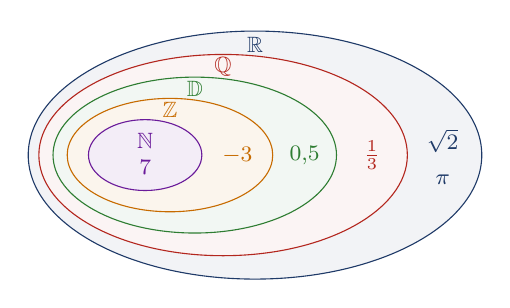
\begin{tikzpicture}[scale=0.9,font=\footnotesize]
\draw[cSec,fill=cSec!6] (0,0) ellipse (3.2 and 1.75);
\draw[cThm,fill=cThm!5] (-0.45,0) ellipse (2.6 and 1.42);
\draw[cRem,fill=cRem!6] (-0.85,0) ellipse (2.0 and 1.1);
\draw[cEx,fill=cEx!7] (-1.2,0) ellipse (1.45 and 0.8);
\draw[cMeth,fill=cMeth!8] (-1.55,0) ellipse (0.8 and 0.5);
\node[cMeth] at (-1.55,0.2){$\mathbb{N}$};
\node[cMeth] at (-1.55,-0.18){$7$};
\node[cEx] at (-1.2,0.64){$\mathbb{Z}$};
\node[cEx] at (-0.25,0){$-3$};
\node[cRem] at (-0.85,0.94){$\mathbb{D}$};
\node[cRem] at (0.7,0){$0{,}5$};
\node[cThm] at (-0.45,1.25){$\mathbb{Q}$};
\node[cThm] at (1.65,0){$\frac{1}{3}$};
\node[cSec] at (0,1.56){$\mathbb{R}$};
\node[cSec] at (2.65,0.2){$\sqrt{2}$};
\node[cSec] at (2.65,-0.35){$\pi$};
\end{tikzpicture}
\end{LTR}}
\end{khassia}

\begin{mithal}[أصغر مجموعة ينتمي إليها عدد]
\begin{itemize}
\item $\sqrt{16}=4$ ، إذن $\sqrt{16}\in\N$. \qquad $\bullet$ $\ \dfrac{-12}{4}=-3\in\Z$ و $-3\notin\N$.
\item $\dfrac{7}{4}=1{,}75=\dfrac{175}{10^{2}}$ ، إذن $\dfrac{7}{4}\in\D$. \qquad $\bullet$ $\ \dfrac{1}{3}=0{,}333\ldots$ ، إذن $\dfrac{1}{3}\in\Q$ و $\dfrac{1}{3}\notin\D$.
\item $-\sqrt{5}\in\R$ لكن $-\sqrt{5}\notin\Q$. \qquad $\bullet$ $\ \dfrac{\sqrt{12}}{\sqrt{3}}=\sqrt{4}=2\in\N$ (نبسط أولًا ثم نحكم!).
\end{itemize}
\end{mithal}

\subsection{متى يكون كسر عددًا عشريًا؟}
\begin{khassia}[مميز الأعداد العشرية]
الكسر $\dfrac{a}{b}$ \textbf{غير القابل للاختزال} ($b>0$) يكون عددًا عشريًا إذا وفقط إذا كان تحليل مقامه $b$ إلى جداء عوامل أولية لا يحتوي إلا على العاملين $2$ و $5$.
\end{khassia}
\begin{mithal}
\begin{itemize}
\item $\dfrac{3}{40}=\dfrac{3}{2^{3}\times5}$ ، إذن \bx{\frac{3}{40}\in\D} (فعلًا $\frac{3}{40}=\frac{75}{1000}=0{,}075$).
\item $\dfrac{21}{75}=\dfrac{7}{25}=\dfrac{7}{5^{2}}$ ، إذن \bx{\frac{21}{75}\in\D} و $\frac{21}{75}=0{,}28$. (المقام $75=3\times5^{2}$ فيه $3$ لكن الكسر يختزل!)
\item $\dfrac{5}{6}=\dfrac{5}{2\times3}$ غير قابل للاختزال ومقامه يحتوي العامل $3$ ، إذن \bx{\frac{5}{6}\notin\D}.
\end{itemize}
\end{mithal}
\begin{khassia}[برهان: $\frac{1}{3}\notin\D$]
نفرض أن $\frac{1}{3}\in\D$ ، أي يوجد $a\in\Z$ و $n\in\N$ بحيث $\frac{1}{3}=\frac{a}{10^{n}}$. إذن $3a=10^{n}=2^{n}\times5^{n}$ ، أي $3$ يقسم $2^{n}\times5^{n}$ ، وهذا مستحيل لأن العوامل الأولية لـ $10^{n}$ هي $2$ و $5$ فقط. \textbf{تناقض}، إذن \bx{\frac{1}{3}\notin\D}.
\end{khassia}

\subsection{الكتابة العشرية الدورية}
\begin{molahada}
كل عدد ناطق له كتابة عشرية \textbf{منتهية} (فهو عشري) أو \textbf{غير منتهية دورية}. وبالعكس، كل كتابة عشرية دورية تمثل عددًا ناطقًا. أما العدد الأصم فكتابته العشرية غير منتهية وغير دورية.
\end{molahada}
\begin{tariqa}[من الكتابة الدورية إلى الكسر]
\begin{enumerate}
\item نسمي $x$ العدد (أو جزأه العشري).
\item نضرب $x$ في $10^{n}$ حيث $n$ عدد أرقام الدور، فيتكرر نفس الجزء الدوري.
\item نطرح طرفًا لطرف فيختفي الجزء غير المنتهي، ثم نحل المعادلة ونختزل الكسر.
\end{enumerate}
\end{tariqa}
\begin{mithal}
\begin{itemize}
\item $x=0{,}363636\ldots$ : الدور $36$ (رقمان): $100x=36{,}3636\ldots$ ، إذن $100x-x=36$ ، أي $99x=36$ و \bx{x=\frac{36}{99}=\frac{4}{11}}.
\item $a=3{,}254254\ldots=3+x$ حيث $x=0{,}254254\ldots$: $1000x=254+x$ ، أي $999x=254$ ، إذن \bx{a=3+\frac{254}{999}=\frac{3251}{999}}.
\item $y=2{,}1555\ldots$ (الدور يبدأ بعد رقم): $10y=21{,}555\ldots$ و $100y=215{,}555\ldots$ ، بالطرح: $90y=194$ ، إذن \bx{y=\frac{194}{90}=\frac{97}{45}}.
\item $z=0{,}999\ldots$: $10z=9+z$ ، أي $9z=9$ و $z=1$. (الكتابة $0{,}999\ldots$ هي كتابة أخرى للعدد $1$.)
\end{itemize}
\end{mithal}

\subsection{البرهان بالخلف: $\sqrt{2}$ عدد أصم}
\begin{tarif}[مبدأ البرهان بالخلف]
لإثبات صحة عبارة $P$:
\begin{enumerate}
\item نفرض أن $P$ خاطئة (نفرض عكسها).
\item نُجري سلسلة من الاستنتاجات الصحيحة.
\item نصل إلى \textbf{تناقض} (مع المعطيات أو مع خاصية معروفة)، فنستنتج أن الفرضية خاطئة وأن $P$ صحيحة.
\end{enumerate}
\end{tarif}
\begin{khassia}[تذكير بالزوجية]
\begin{itemize}
\item العدد الزوجي يكتب $2k$ ، والعدد الفردي يكتب $2k+1$ حيث $k\in\Z$.
\item $(2k)^{2}=2(2k^{2})$ زوجي و $(2k+1)^{2}=2(2k^{2}+2k)+1$ فردي؛ إذن: \bxt{إذا كان $p^{2}$ زوجيًا فإن $p$ زوجي}.
\end{itemize}
\end{khassia}
\begin{mithal}[مثال مرجعي: $\sqrt{2}\notin\Q$]
نفرض أن $\sqrt{2}=\dfrac{p}{q}$ حيث $\dfrac{p}{q}$ كسر \textbf{غير قابل للاختزال} ($p,q\in\N^{*}$).
\begin{itemize}
\item $2=\dfrac{p^{2}}{q^{2}}$ ، ومنه $p^{2}=2q^{2}$ ، إذن $p^{2}$ زوجي ومنه $p$ زوجي: $p=2k$.
\item بالتعويض: $4k^{2}=2q^{2}$ ، أي $q^{2}=2k^{2}$ ، إذن $q^{2}$ زوجي ومنه $q$ زوجي.
\item $p$ و $q$ زوجيان، فالكسر $\frac{p}{q}$ يقبل الاختزال على $2$: \textbf{تناقض}. إذن \bx{\sqrt{2}\notin\Q}.
\end{itemize}
\end{mithal}
\begin{molahada}[نتيجة مفيدة]
إذا كان $r$ ناطقًا و $x$ أصمّ فإن $r+x$ أصمّ (و $rx$ أصم إذا $r\neq0$). مثلًا: لو كان $1+\sqrt{2}=r\in\Q$ لكان $\sqrt{2}=r-1\in\Q$: تناقض. إذن $1+\sqrt{2}\notin\Q$.
\end{molahada}

\subsection{الأعداد القابلة للإنشاء}
\begin{tarif}
نقول عن عدد حقيقي موجب $x$ إنه \textbf{قابل للإنشاء} إذا أمكن رسم قطعة مستقيمة طولها $x$ باستعمال المسطرة غير المدرجة والمدور فقط، انطلاقًا من قطعة طولها $1$.
\end{tarif}
\begin{khassia}[طرق الإنشاء]
\RL{0.6}{%
\begin{itemize}
\item \textbf{مبرهنة فيثاغورس:} قطر مربع طول ضلعه $1$ هو $\sqrt{2}$؛ ووتر مثلث قائم ضلعاه $1$ و $\sqrt{n}$ هو $\sqrt{n+1}$ (حلزون فيثاغورس).
\item \textbf{مبرهنة طالس:} تسمح بإنشاء $\frac{a}{b}$ وبتقسيم قطعة إلى أجزاء متقايسة.
\item \textbf{العلاقة المترية في المثلث القائم:} $AH^{2}=HB\times HC$ تسمح بإنشاء $\sqrt{a}$.
\end{itemize}}{0.37}{%
\begin{LTR}\centering
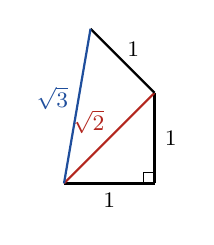
\begin{tikzpicture}[scale=1.15,font=\footnotesize]
\coordinate (O) at (0,0);
\coordinate (A) at (1,0);
\coordinate (B) at (1,1);
\coordinate (C) at ($(B)+(-0.7071,0.7071)$);
\draw[thick] (O)--(A) node[midway,below]{$1$};
\draw[thick] (A)--(B) node[midway,right]{$1$};
\draw[thick,cThm] (O)--(B) node[midway,above left=-2pt]{$\sqrt{2}$};
\draw[thick] (B)--(C) node[midway,above right=-2pt]{$1$};
\draw[thick,cDef] (O)--(C) node[pos=0.55,left]{$\sqrt{3}$};
\draw (A)++(-0.12,0)--++(0,0.12)--++(0.12,0);
\end{tikzpicture}
\end{LTR}}
\end{khassia}

%================================================================
\section{الحساب في $\N$: القواسم والأعداد الأولية}
\begin{tarif}[قاسم، مضاعف]
$a$ و $b$ عددان طبيعيان، $b\neq0$. نقول إن $b$ \textbf{يقسم} $a$ (أو $a$ مضاعف لـ $b$) إذا وُجد $k\in\N$ بحيث $a=k\times b$.
مثال: $91=7\times13$ ، إذن $7$ و $13$ قاسمان لـ $91$.
\end{tarif}
\begin{tarif}[العدد الأولي]
العدد الطبيعي $p$ \textbf{أولي} إذا كان يقبل قاسمين بالضبط: $1$ ونفسه. (العدد $1$ ليس أوليًا.)\par
الأعداد الأولية الأصغر من $50$: \ $2$ ، $3$ ، $5$ ، $7$ ، $11$ ، $13$ ، $17$ ، $19$ ، $23$ ، $29$ ، $31$ ، $37$ ، $41$ ، $43$ ، $47$.
\end{tarif}
\begin{tariqa}[كيف نعرف أن عددًا $n$ أولي؟]
نقسم $n$ على الأعداد الأولية $p$ بالترتيب ما دام $p^{2}\leqslant n$ (أي $p\leqslant\sqrt{n}$). إذا لم يقبل $n$ القسمة على أي منها فهو أولي.
\end{tariqa}
\begin{mithal}
\begin{itemize}
\item $113$: \ $\sqrt{113}\approx10{,}6$ ، و $113$ لا يقبل القسمة على $2$ ، $3$ ، $5$ ، $7$ ، إذن \bxt{$113$ أولي}.
\item $221$: \ $\sqrt{221}\approx14{,}9$ ؛ لا يقبل القسمة على $2$ ، $3$ ، $5$ ، $7$ ، $11$ ، لكن $221=13\times17$ ، إذن \bxt{$221$ ليس أوليًا}.
\end{itemize}
\end{mithal}
\begin{khassia}[التحليل إلى جداء عوامل أولية]
كل عدد طبيعي $n\geqslant2$ يكتب بطريقة وحيدة (دون اعتبار الترتيب) على شكل جداء عوامل أولية:
$n=p_{1}^{\alpha_{1}}\times p_{2}^{\alpha_{2}}\times\cdots\times p_{k}^{\alpha_{k}}$ ، وعدد قواسمه هو $(\alpha_{1}+1)(\alpha_{2}+1)\cdots(\alpha_{k}+1)$.
\end{khassia}
\begin{mithal}
\RL{0.62}{%
$360=2^{3}\times3^{2}\times5$ \quad (القسمة المتتالية على $2$ ، $2$ ، $2$ ، $3$ ، $3$ ، $5$).\par
عدد قواسم $360$: \ $(3+1)(2+1)(1+1)=\bx{24}$.\par
$\sqrt{360}=\sqrt{2^{2}\times3^{2}\times10}=6\sqrt{10}$.}{0.33}{%
\begin{LTR}\centering\small
\begin{tabular}{r|l}
$360$ & $2$\\ $180$ & $2$\\ $90$ & $2$\\ $45$ & $3$\\ $15$ & $3$\\ $5$ & $5$\\ $1$ &
\end{tabular}
\end{LTR}}
\end{mithal}

\subsection{القاسم المشترك الأكبر والمضاعف المشترك الأصغر}
\begin{tarif}
\begin{itemize}
\item $\pgcd(a;b)$: أكبر قاسم مشترك لـ $a$ و $b$؛ نأخذ \textbf{العوامل المشتركة} بأصغر أُس.
\item $\ppcm(a;b)$: أصغر مضاعف مشترك غير معدوم؛ نأخذ \textbf{كل العوامل} بأكبر أُس.
\item $a$ و $b$ \textbf{أوليان فيما بينهما} إذا كان $\pgcd(a;b)=1$.
\end{itemize}
\end{tarif}
\begin{khassia}
\begin{itemize}
\item $\pgcd(a;b)\times\ppcm(a;b)=a\times b$.
\item \textbf{خوارزمية إقليدس:} $\pgcd(a;b)=\pgcd(b;r)$ حيث $r$ باقي القسمة الإقليدية لـ $a$ على $b$؛ و $\pgcd$ هو آخر باقٍ غير معدوم.
\item الكسر $\frac{a}{b}$ غير قابل للاختزال إذا وفقط إذا كان $\pgcd(a;b)=1$؛ ولاختزال كسر نقسم بسطه ومقامه على $\pgcd$.
\end{itemize}
\end{khassia}
\begin{mithal}[بالتحليل]
$84=2^{2}\times3\times7$ \quad و \quad $90=2\times3^{2}\times5$.
\begin{itemize}
\item $\pgcd(84;90)=2\times3=\bx{6}$ ، \quad $\ppcm(84;90)=2^{2}\times3^{2}\times5\times7=\bx{1260}$.
\item التحقق: $6\times1260=7560=84\times90$ ، \quad الاختزال: $\dfrac{84}{90}=\dfrac{84\div6}{90\div6}=\bx{\frac{14}{15}}$.
\end{itemize}
\end{mithal}
\begin{mithal}[بخوارزمية إقليدس: $\pgcd(1071;462)$]
\begin{LTR}\centering
\renewcommand{\arraystretch}{1.2}
\begin{tabular}{|c|c|c|c|}\hline
\rowcolor{cSec!12}$a$ & $b$ & $a=bq+r$ & $r$\\\hline
$1071$ & $462$ & $1071=462\times2+147$ & $147$\\\hline
$462$ & $147$ & $462=147\times3+21$ & $21$\\\hline
$147$ & $21$ & $147=21\times7+0$ & $0$\\\hline
\end{tabular}
\end{LTR}
\par آخر باقٍ غير معدوم هو $21$ ، إذن \bx{\pgcd(1071;462)=21} و $\dfrac{462}{1071}=\dfrac{462\div21}{1071\div21}=\bx{\frac{22}{51}}$.
\end{mithal}

%================================================================
\section{القوى والجذور التربيعية}
\begin{tarif}[القوى]
من أجل كل عدد حقيقي $a$ وكل عدد طبيعي $n\geqslant1$:
\[ a^{n}=\underbrace{a\times a\times\cdots\times a}_{n\ \text{مرة}}\qquad;\qquad a^{0}=1\quad(a\neq0)\qquad;\qquad a^{-n}=\frac{1}{a^{n}}\quad(a\neq0) \]
\end{tarif}
\begin{khassia}[قواعد الحساب على القوى ($a\neq0$ ، $b\neq0$ ، $m,n\in\Z$)]
\begin{LTR}\centering
\renewcommand{\arraystretch}{1.6}
\begin{tabular}{|c|c|c|}\hline
$a^{m}\times a^{n}=a^{m+n}$ & $\dfrac{a^{m}}{a^{n}}=a^{m-n}$ & $\left(a^{m}\right)^{n}=a^{m\times n}$\\\hline
$(a\times b)^{n}=a^{n}\times b^{n}$ & $\left(\dfrac{a}{b}\right)^{n}=\dfrac{a^{n}}{b^{n}}$ & \ar{$(-a)^{n}=a^{n}$ ($n$ زوجي) ، $(-a)^{n}=-a^{n}$ ($n$ فردي)}\\\hline
\end{tabular}
\end{LTR}
\end{khassia}
\begin{mithal}[تبسيط]
\begin{itemize}
\item $A=\dfrac{\left(2^{3}\times3^{-2}\right)^{2}\times3^{5}}{2^{4}}=\dfrac{2^{6}\times3^{-4}\times3^{5}}{2^{4}}=2^{6-4}\times3^{-4+5}=2^{2}\times3=\bx{12}$.
\item $B=\dfrac{(-2)^{5}\times4^{-2}}{8^{-1}}=\dfrac{-2^{5}\times2^{-4}}{2^{-3}}=-2^{5-4+3}=-2^{4}=\bx{-16}$.
\item انتبه: $(-2)^{4}=16$ بينما $-2^{4}=-(2^{4})=-16$.
\end{itemize}
\end{mithal}

\begin{tarif}[الجذر التربيعي]
من أجل كل عدد حقيقي موجب $a$ ، $\sqrt{a}$ هو العدد الحقيقي \textbf{الموجب} الذي مربعه $a$:\quad $\left(\sqrt{a}\right)^{2}=a$ و $\sqrt{a}\geqslant0$.
\end{tarif}
\begin{khassia}[قواعد الحساب على الجذور]
\begin{LTR}\centering
\renewcommand{\arraystretch}{1.6}
\begin{tabular}{|c|c|c|}\hline
$\sqrt{a\times b}=\sqrt{a}\times\sqrt{b}$ \ $(a,b\geqslant0)$ & $\sqrt{\dfrac{a}{b}}=\dfrac{\sqrt{a}}{\sqrt{b}}$ \ $(a\geqslant0,\ b>0)$ & $\sqrt{a^{2}}=|a|$ \ $(a\in\mathbb{R})$\\\hline
\end{tabular}
\end{LTR}
\par\smallskip
\textbf{تنبيه:} $\sqrt{a+b}\neq\sqrt{a}+\sqrt{b}$ عمومًا. مثلًا: $\sqrt{9+16}=\sqrt{25}=5$ بينما $\sqrt{9}+\sqrt{16}=7$.
\end{khassia}
\begin{tariqa}[التخلص من الجذر في المقام: الضرب في المرافق]
مرافق $\sqrt{a}-\sqrt{b}$ هو $\sqrt{a}+\sqrt{b}$ ، وجداؤهما $a-b$ (لا جذر فيه):
\[ \frac{1}{\sqrt{a}}=\frac{\sqrt{a}}{a}\qquad;\qquad \frac{1}{\sqrt{a}-\sqrt{b}}=\frac{\sqrt{a}+\sqrt{b}}{a-b}\qquad;\qquad \frac{1}{\sqrt{a}+b}=\frac{\sqrt{a}-b}{a-b^{2}} \]
\end{tariqa}
\begin{mithal}
\begin{itemize}
\item $\sqrt{75}-2\sqrt{12}+\sqrt{27}=\sqrt{25\times3}-2\sqrt{4\times3}+\sqrt{9\times3}=5\sqrt{3}-4\sqrt{3}+3\sqrt{3}=\bx{4\sqrt{3}}$.
\item $\left(\sqrt{3}-1\right)^{2}=3-2\sqrt{3}+1=\bx{4-2\sqrt{3}}$ ، ومنه $\sqrt{4-2\sqrt{3}}=\left|\sqrt{3}-1\right|=\bx{\sqrt{3}-1}$ (لأن $\sqrt{3}>1$).
\item $\dfrac{2}{\sqrt{5}-1}=\dfrac{2\left(\sqrt{5}+1\right)}{\left(\sqrt{5}-1\right)\left(\sqrt{5}+1\right)}=\dfrac{2\left(\sqrt{5}+1\right)}{5-1}=\bx{\frac{\sqrt{5}+1}{2}}$.
\item $\dfrac{1}{\sqrt{3}+\sqrt{2}}=\dfrac{\sqrt{3}-\sqrt{2}}{3-2}=\bx{\sqrt{3}-\sqrt{2}}$.
\end{itemize}
\end{mithal}

\subsection{الكتابة العلمية ورتبة المقدار}
\begin{tarif}[الكتابة العلمية]
الكتابة العلمية لعدد عشري غير معدوم هي كتابته على الشكل $a\times10^{n}$ أو $-a\times10^{n}$ حيث \bx{1\leqslant a<10} و $n\in\Z$.
\end{tarif}
\begin{mithal}
\begin{itemize}
\item $128\,000\,000=\bx{1{,}28\times10^{8}}$ \qquad ؛ \qquad $-0{,}000\,000\,000\,75=\bx{-7{,}5\times10^{-10}}$.
\item $32{,}1\times10^{-5}$ ليست كتابة علمية لأن $32{,}1>10$؛ كتابتها العلمية: $3{,}21\times10^{1}\times10^{-5}=\bx{3{,}21\times10^{-4}}$.
\item $\dfrac{3\times10^{4}\times5\times10^{-7}}{2\times10^{-5}}=\dfrac{15}{2}\times10^{4-7+5}=7{,}5\times10^{2}=\bx{750}$.
\end{itemize}
\end{mithal}
\begin{tarif}[رتبة المقدار]
رتبة مقدار عدد كتابته العلمية $a\times10^{n}$ هي $k\times10^{n}$ حيث $k$ مدوّر $a$ إلى الوحدة. ولإيجاد رتبة مقدار جداء أو حاصل قسمة نحسب برتب مقادير الأعداد.
\end{tarif}
\begin{mithal}
$\dfrac{82{,}6\times10^{3}}{47\times10^{-8}}=\dfrac{8{,}26\times10^{4}}{4{,}7\times10^{-7}}$ ؛ رتبة المقدار: $\dfrac{8\times10^{4}}{5\times10^{-7}}=1{,}6\times10^{11}$ ، أي \bx{2\times10^{11}}. (القيمة الفعلية $\approx1{,}76\times10^{11}$.)
\end{mithal}

%================================================================
\section{الحساب الحرفي والبرهان على صحة مساواة}
\begin{khassia}[أولويات العمليات]
\begin{enumerate}
\item الحسابات داخل الأقواس.
\item القوى والجذور التربيعية.
\item الضرب والقسمة حسب ترتيب كتابتها.
\item الجمع والطرح حسب ترتيب كتابتها.
\end{enumerate}
مثال: $2+3\times4^{2}=2+3\times16=50$ \ بينما \ $(2+3)\times4^{2}=80$.
\end{khassia}
\begin{khassia}[المتطابقات الشهيرة]
من أجل كل عددين حقيقيين $a$ و $b$:
\[ \bx{(a+b)^{2}=a^{2}+2ab+b^{2}}\qquad \bx{(a-b)^{2}=a^{2}-2ab+b^{2}}\qquad \bx{(a-b)(a+b)=a^{2}-b^{2}} \]
تستعمل للنشر (من اليسار إلى اليمين) وللتحليل (من اليمين إلى اليسار).
\end{khassia}
\begin{mithal}[نشر وتحليل]
\begin{itemize}
\item $\left(2\sqrt{3}+1\right)^{2}=12+4\sqrt{3}+1=\bx{13+4\sqrt{3}}$.
\item $9x^{2}-25=(3x)^{2}-5^{2}=\bx{(3x-5)(3x+5)}$ \ ؛ \ $x^{2}-6x+9=\bx{(x-3)^{2}}$.
\item $a^{2}+1-2a=(a-1)^{2}\geqslant0$ ، إذن من أجل كل عدد حقيقي $a$: \bx{a^{2}+1\geqslant2a}.
\end{itemize}
\end{mithal}
\begin{tariqa}[ثلاث طرق للبرهان على أن $A=B$]
\begin{enumerate}
\item ننطلق من أحد الطرفين ونحوّل كتابته بقواعد الحساب حتى نصل إلى الطرف الآخر.
\item نحوّل كتابة كل من $A$ و $B$ حتى نصل إلى نفس العبارة $C$.
\item نبرهن أن $A-B=0$.
\end{enumerate}
وإذا كان $A$ و $B$ \textbf{موجبين} يمكن أيضًا البرهان على أن $A^{2}=B^{2}$.
\end{tariqa}
\begin{mithal}[الطريقة 3]
البرهان على أن $\dfrac{1+\sqrt{5}}{2}=\dfrac{3+\sqrt{5}}{1+\sqrt{5}}$:
\[ \frac{1+\sqrt{5}}{2}-\frac{3+\sqrt{5}}{1+\sqrt{5}}=\frac{\left(1+\sqrt{5}\right)^{2}-2\left(3+\sqrt{5}\right)}{2\left(1+\sqrt{5}\right)}=\frac{6+2\sqrt{5}-6-2\sqrt{5}}{2\left(1+\sqrt{5}\right)}=\bx{0} \]
\end{mithal}
\begin{mithal}[بالمربعين (عددان موجبان)]
البرهان على أن $\sqrt{8+2\sqrt{7}}=\sqrt{7}+1$: \ الطرفان موجبان و
\[ \left(\sqrt{7}+1\right)^{2}=7+2\sqrt{7}+1=8+2\sqrt{7}=\left(\sqrt{8+2\sqrt{7}}\right)^{2} \]
لهما نفس المربع وهما موجبان، إذن \bx{\sqrt{8+2\sqrt{7}}=\sqrt{7}+1}.
\end{mithal}

%================================================================
\section{المقارنة والترتيب في $\R$}
\begin{tarif}
$a$ و $b$ عددان حقيقيان:
\[ a<b\iff a-b<0\qquad;\qquad a>b\iff a-b>0\qquad;\qquad a\geqslant b\iff a-b\geqslant0 \]
مقارنة عددين $a$ و $b$ معناها التصريح بإحدى الحالات: $a<b$ أو $a=b$ أو $a>b$.
\end{tarif}
\begin{tariqa}[طرق المقارنة]
\begin{enumerate}
\item \textbf{دراسة إشارة الفرق} $a-b$ (الطريقة العامة).
\item \textbf{مقارنة المربعين} إذا كان العددان موجبين: $a^{2}<b^{2}\iff a<b$.
\item \textbf{مقارنة المقلوبين} إذا كان العددان من نفس الإشارة: $a<b\iff\frac{1}{a}>\frac{1}{b}$.
\item \textbf{مقارنة حاصل القسمة بـ $1$} إذا كان العددان موجبين تمامًا: $\frac{a}{b}<1\iff a<b$.
\item \textbf{عدد وسيط} (التعدي): إذا كان $a\leqslant c$ و $c\leqslant b$ فإن $a\leqslant b$.
\end{enumerate}
\end{tariqa}
\begin{mithal}[تطبيق كل طريقة]
\begin{itemize}
\item \textbf{الفرق:} $\dfrac{7}{9}-\dfrac{11}{14}=\dfrac{98-99}{126}=-\dfrac{1}{126}<0$ ، إذن \bx{\frac{7}{9}<\frac{11}{14}}.
\item \textbf{المربعان:} $\left(2\sqrt{3}\right)^{2}=12$ و $\left(3\sqrt{2}\right)^{2}=18$ ، و $12<18$ والعددان موجبان، إذن \bx{2\sqrt{3}<3\sqrt{2}}.
\item \textbf{المربعان:} $\left(\sqrt{3}+\sqrt{5}\right)^{2}=8+2\sqrt{15}$ و $\left(\sqrt{2}+\sqrt{6}\right)^{2}=8+2\sqrt{12}$ ، و $\sqrt{15}>\sqrt{12}$ ، إذن \bx{\sqrt{3}+\sqrt{5}>\sqrt{2}+\sqrt{6}}.
\item \textbf{المقلوبان:} $\sqrt{7}<\sqrt{8}$ (عددان موجبان) ، إذن \bx{\frac{1}{\sqrt{7}}>\frac{1}{\sqrt{8}}}.
\item \textbf{حاصل القسمة:} $\dfrac{1/(\sqrt{5}-2)}{\sqrt{5}+2}=\dfrac{1}{(\sqrt{5}-2)(\sqrt{5}+2)}=\dfrac{1}{5-4}=1$ ، إذن \bx{\frac{1}{\sqrt{5}-2}=\sqrt{5}+2}.
\end{itemize}
\end{mithal}

\subsection{الترتيب والعمليات}
\begin{khassia}[$a$ ، $b$ ، $c$ ، $d$ أعداد حقيقية]
\begin{center}
\renewcommand{\arraystretch}{1.45}
\begin{tabular}{|>{\centering\arraybackslash}p{0.27\textwidth}|>{\centering\arraybackslash}p{0.38\textwidth}|>{\centering\arraybackslash}p{0.2\textwidth}|}\hline
\rowcolor{cSec!12}\textbf{مثال} & \textbf{الخاصية} & \textbf{العملية}\\\hline
$a-3\leqslant b-3\Rightarrow a\leqslant b$ & $a\leqslant b\iff a+c\leqslant b+c$ & جمع عدد\\\hline
$a\leqslant5$ و $b\leqslant-3\Rightarrow a+b\leqslant2$ & $a\leqslant b$ و $c\leqslant d\Rightarrow a+c\leqslant b+d$ & جمع متباينتين\\\hline
$2\leqslant3\Rightarrow0{,}02\leqslant0{,}03$ & $c>0$: \ $a\leqslant b\iff ac\leqslant bc$ & الضرب في $c>0$\\\hline
$2<5\Rightarrow-6>-15$ & $c<0$: \ $a\leqslant b\iff ac\geqslant bc$ (يتغير الاتجاه) & الضرب في $c<0$\\\hline
$0<a\leqslant2$ و $0<b\leqslant5\Rightarrow ab\leqslant10$ & $0\leqslant a\leqslant b$ و $0\leqslant c\leqslant d\Rightarrow ac\leqslant bd$ & ضرب متباينتين (أعداد موجبة)\\\hline
$-4<-2\Rightarrow16>4$ & $0\leqslant a\leqslant b\iff a^{2}\leqslant b^{2}$ \par $a\leqslant b\leqslant0\iff a^{2}\geqslant b^{2}$ & التربيع\\\hline
$2<3\Rightarrow\sqrt{2}<\sqrt{3}$ & $0\leqslant a\leqslant b\iff\sqrt{a}\leqslant\sqrt{b}$ & الجذر التربيعي\\\hline
$2<5\Rightarrow\frac{1}{2}>\frac{1}{5}$ & $a$ و $b$ من نفس الإشارة: \par $a\leqslant b\iff\frac{1}{a}\geqslant\frac{1}{b}$ & المقلوب\\\hline
\end{tabular}
\end{center}
\textbf{تنبيه:} لا نطرح ولا نقسم متباينتين طرفًا لطرف.
\end{khassia}

\begin{khassia}[مقارنة $a$ ، $a^{2}$ ، $a^{3}$ ، $\sqrt{a}$ ، $\frac{1}{a}$ ($a>0$)]
\begin{itemize}
\item إذا كان $0<a<1$: \quad \bx{a^{3}<a^{2}<a<\sqrt{a}<1<\frac{1}{a}}.
\item إذا كان $a>1$: \quad \bx{\frac{1}{a}<1<\sqrt{a}<a<a^{2}<a^{3}}.
\end{itemize}
\textbf{البرهان} (الحالة $0<a<1$):
\begin{itemize}
\item بضرب $a<1$ في $a>0$: $a^{2}<a$؛ وبضربها في $a^{2}>0$: $a^{3}<a^{2}$.
\item $a-\sqrt{a}=\sqrt{a}\left(\sqrt{a}-1\right)<0$ لأن $\sqrt{a}>0$ و $\sqrt{a}<1$؛ إذن $a<\sqrt{a}$.
\item $\frac{1}{a}>1$ لأن $0<a<1$ (المقلوب يغيّر الاتجاه).
\end{itemize}
\par\smallskip
\begin{LTR}\centering
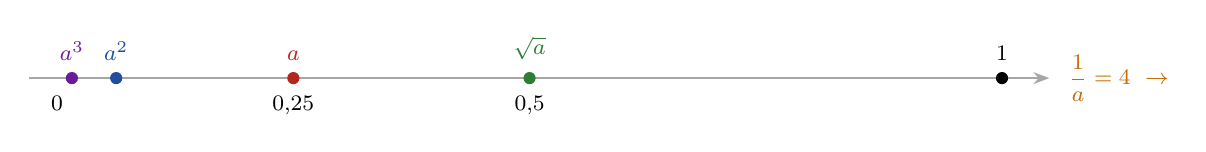
\begin{tikzpicture}[x=12cm,font=\footnotesize]
\draw[nl] (-0.03,0)--(1.05,0);
\foreach \x/\l/\c in {0.015625/a^{3}/cMeth,0.0625/a^{2}/cDef,0.25/a/cThm,0.5/\sqrt{a}/cRem,1/1/black}
 {\fill[\c] (\x,0) circle (2.2pt); \node[above=3pt,\c] at (\x,0){$\l$};}
\node[below=3pt] at (0,0){$0$};
\node[below=3pt] at (0.25,0){$0{,}25$};
\node[below=3pt] at (0.5,0){$0{,}5$};

\node[cEx,right] at (1.06,0){$\dfrac{1}{a}=4\ \to$};
\end{tikzpicture}
\end{LTR}
\par مثال: من أجل $a=0{,}25$: \ $a^{3}\approx0{,}016<a^{2}=0{,}0625<a=0{,}25<\sqrt{a}=0{,}5<1<\frac{1}{a}=4$.
\end{khassia}

%================================================================
\section{الحصر والقيم المقربة}
\begin{tarif}[حصر عدد حقيقي]
حصر عدد حقيقي $x$ يعني إيجاد عددين $a$ و $b$ بحيث $a\leqslant x\leqslant b$. العدد $b-a$ يسمى \textbf{سعة الحصر}.\par
مثال: $1{,}41\leqslant\sqrt{2}\leqslant1{,}42$ حصر لـ $\sqrt{2}$ سعته $10^{-2}$.
\end{tarif}
\begin{khassia}[العمليات على الحصر: إذا كان $a\leqslant x\leqslant b$ و $c\leqslant y\leqslant d$]
\begin{center}
\renewcommand{\arraystretch}{1.7}
\begin{tabular}{|>{\centering\arraybackslash}p{0.5\textwidth}|>{\centering\arraybackslash}p{0.3\textwidth}|}\hline
\rowcolor{cSec!12}\textbf{النتيجة} & \textbf{المطلوب}\\\hline
$a+c\leqslant x+y\leqslant b+d$ & المجموع $x+y$\\\hline
$-d\leqslant-y\leqslant-c$ \ ثم \ $a-d\leqslant x-y\leqslant b-c$ & الفرق $x-y$\\\hline
$ac\leqslant xy\leqslant bd$ \quad ($a\geqslant0$ ، $c\geqslant0$) & الجداء $xy$\\\hline
$\frac{1}{b}\leqslant\frac{1}{x}\leqslant\frac{1}{a}$ \quad ($a>0$) & المقلوب $\frac{1}{x}$\\\hline
$\frac{a}{d}\leqslant\frac{x}{y}\leqslant\frac{b}{c}$ \quad ($a\geqslant0$ ، $c>0$) & حاصل القسمة $\frac{x}{y}=x\times\frac{1}{y}$\\\hline
$a^{2}\leqslant x^{2}\leqslant b^{2}$ \quad ($a\geqslant0$) & المربع $x^{2}$\\\hline
\end{tabular}
\end{center}
\textbf{تنبيه:} لحصر $x-y$ نحصر $-y$ أولًا ثم نجمع؛ ولحصر $\frac{x}{y}$ نحصر $\frac{1}{y}$ أولًا ثم نضرب.
\end{khassia}
\begin{mithal}[$2\leqslant x\leqslant3$ و $1\leqslant y\leqslant2$]
\begin{itemize}
\item \textbf{المجموع:} $2+1\leqslant x+y\leqslant3+2$ ، أي \bx{3\leqslant x+y\leqslant5}.
\item \textbf{الفرق:} $-2\leqslant-y\leqslant-1$ ، ومنه $2-2\leqslant x-y\leqslant3-1$ ، أي \bx{0\leqslant x-y\leqslant2}.
\item \textbf{الجداء} (حدود موجبة): $2\times1\leqslant xy\leqslant3\times2$ ، أي \bx{2\leqslant xy\leqslant6}.
\item \textbf{حاصل القسمة:} $\frac{1}{2}\leqslant\frac{1}{y}\leqslant1$ ، ومنه $2\times\frac{1}{2}\leqslant\frac{x}{y}\leqslant3\times1$ ، أي \bx{1\leqslant\frac{x}{y}\leqslant3}.
\item \textbf{مجموع المربعين:} $4\leqslant x^{2}\leqslant9$ و $1\leqslant y^{2}\leqslant4$ ، ومنه \bx{5\leqslant x^{2}+y^{2}\leqslant13}.
\item \textbf{المقلوب:} $3\leqslant x+y\leqslant5$ (أعداد موجبة) ، ومنه \bx{\frac{1}{5}\leqslant\frac{1}{x+y}\leqslant\frac{1}{3}}.
\end{itemize}
\end{mithal}
\begin{molahada}[حالة حدود سالبة]
إذا كان $-3<x<-2$ (عدد سالب) فإن $4<x^{2}<9$ (التربيع يغيّر الاتجاه للسالبة). أما إذا كان $-3<x<2$ (تغير الإشارة) فلا نربّع الطرفين: نفصل الحالتين فنجد $0\leqslant x^{2}<9$.
\end{molahada}

\subsection{القيم المقربة والتدوير}
\begin{tarif}[القيمة المقربة]
$a$ عدد حقيقي و $d$ عدد عشري. نقول إن $d$ \textbf{قيمة مقربة للعدد $a$ إلى $10^{-n}$} إذا كان $|a-d|\leqslant10^{-n}$.
\begin{itemize}
\item إذا كان $d\leqslant a$ فهي قيمة مقربة \textbf{بالنقصان}؛ وإذا كان $d\geqslant a$ فهي قيمة مقربة \textbf{بالزيادة}.
\item من الحصر $1{,}414<\sqrt{2}<1{,}415$: \ $1{,}414$ قيمة مقربة بالنقصان و $1{,}415$ قيمة مقربة بالزيادة إلى $10^{-3}$.
\item \textbf{المدوّر} إلى $10^{-n}$ هو أقرب القيمتين المقربتين (بالنقصان أو بالزيادة) إلى $10^{-n}$.
\end{itemize}
\end{tarif}
\begin{tariqa}[التدوير إلى الرتبة $10^{-p}$]
ليكن $d$ الرقم العشري الذي رتبته $10^{-(p+1)}$ (الرقم الموالي):
\begin{itemize}
\item إذا كان $d\geqslant5$ نضيف $1$ إلى الرقم ذي الرتبة $10^{-p}$؛
\item إذا كان $d<5$ نترك الرقم ذا الرتبة $10^{-p}$ كما هو، ونحذف ما بعده.
\end{itemize}
\end{tariqa}
\begin{mithal}
\begin{itemize}
\item $a=5{,}678\,234\,56$: المدوّر إلى الوحدة $6$ ، إلى $10^{-1}$: $5{,}7$ ، إلى $10^{-2}$: $5{,}68$ ، إلى $10^{-3}$: $5{,}678$.
\item $\pi=3{,}141\,59\ldots$: \ $3{,}141<\pi<3{,}142$ ؛ القيمة المقربة بالنقصان إلى $10^{-3}$ هي $3{,}141$ ، والمدوّر إلى $10^{-3}$ هو $3{,}142$.
\item من $2{,}23<\sqrt{5}<2{,}24$: $2{,}23$ قيمة مقربة بالنقصان و $2{,}24$ قيمة مقربة بالزيادة لـ $\sqrt{5}$ إلى $10^{-2}$.
\end{itemize}
\end{mithal}

%================================================================
\origNeedspace{30\baselineskip}
\section{المجالات}
\begin{tarif}[أنواع المجالات ($a<b$)]
\begin{center}
\renewcommand{\arraystretch}{1.25}
\begin{tabular}{|>{\centering\arraybackslash}m{0.17\textwidth}|>{\centering\arraybackslash}m{0.25\textwidth}|>{\centering\arraybackslash}m{0.17\textwidth}|>{\centering\arraybackslash}m{0.15\textwidth}|}\hline
\rowcolor{cSec!12}\textbf{النوع} & \textbf{التمثيل على المستقيم} & \textbf{المتباينة} & \textbf{المجال}\\\hline
مغلق & \NLseg{a}{b}{[}{]} & $a\leqslant x\leqslant b$ & $[a;b]$\\\hline
مفتوح & \NLseg{a}{b}{]}{[} & $a<x<b$ & $]a;b[$\\\hline
نصف مفتوح & \NLseg{a}{b}{[}{[} & $a\leqslant x<b$ & $[a;b[$\\\hline
نصف مفتوح & \NLseg{a}{b}{]}{]} & $a<x\leqslant b$ & $]a;b]$\\\hline
غير محدود & \NLright{a}{[} & $x\geqslant a$ & $[a;+\infty[$\\\hline
غير محدود & \NLright{a}{]} & $x>a$ & $]a;+\infty[$\\\hline
غير محدود & \NLleft{b}{]} & $x\leqslant b$ & $]-\infty;b]$\\\hline
غير محدود & \NLleft{b}{[} & $x<b$ & $]-\infty;b[$\\\hline
\end{tabular}
\end{center}
$\R=\,]-\infty;+\infty[$ \quad ؛ \quad $\R_{+}=[0;+\infty[$ \quad ؛ \quad $\R_{-}=\,]-\infty;0]$ \quad ؛ \quad $\R_{+}^{*}=\,]0;+\infty[$.\par
\textbf{تنبيه:} الرمز $\infty$ يكون دائمًا من جهة مفتوحة. \ العدد $\frac{a+b}{2}$ هو \textbf{مركز} المجال و $\frac{b-a}{2}$ \textbf{نصف قطره} و $b-a$ \textbf{طوله} (سعته).
\end{tarif}

\begin{tarif}[التقاطع والاتحاد]
\begin{itemize}
\item $I\cap J$: مجموعة الأعداد التي تنتمي إلى $I$ \textbf{و} إلى $J$ معًا (الجزء المشترك في التمثيل).
\item $I\cup J$: مجموعة الأعداد التي تنتمي إلى $I$ \textbf{أو} إلى $J$ (كل الجزء الملوّن).
\end{itemize}
\end{tarif}
\begin{tariqa}
نمثل المجالين على نفس المستقيم العددي بلونين مختلفين (على مستويين)، ثم نقرأ الجزء المشترك ($\cap$) أو كل الجزء الملوّن ($\cup$) مع الانتباه لطبيعة كل طرف (مفتوح أو مغلق).
\end{tariqa}
\begin{mithal}[{$I=[-2;5[$ و $J=\,]1;+\infty[$}]
\begin{LTR}\centering
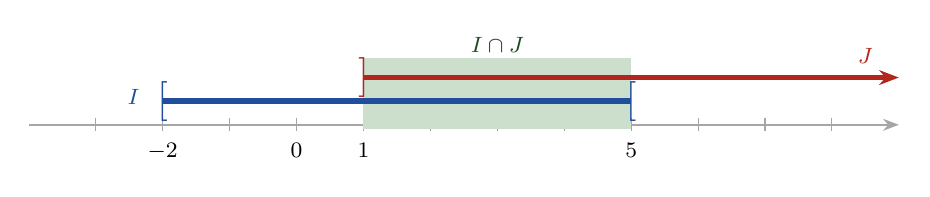
\begin{tikzpicture}[x=0.85cm,font=\footnotesize]
\draw[nl] (-4,0)--(9,0);
\foreach \t in {-3,...,8}\draw[tk] (\t,0.08)--(\t,-0.08);
\foreach \t in {-2,0,1,5}\node[lab] at (\t,0){$\t$};
\fill[cRem!25] (1,-0.05) rectangle (5,0.85);
\draw[line width=2pt,cDef] (-2,0.3)--(5,0.3);
\node[cDef,font=\Large] at (-2,0.3){$[$}; \node[cDef,font=\Large] at (5,0.3){$[$};
\node[cDef,left] at (-2.2,0.35){$I$};
\draw[line width=2pt,cThm,-{Stealth[length=2.5mm]}] (1,0.6)--(9,0.6);
\node[cThm,font=\Large] at (1,0.6){$]$};
\node[cThm,above] at (8.5,0.65){$J$};
\node[cRem!60!black,above] at (3,0.8){$I\cap J$};
\end{tikzpicture}
\end{LTR}
\par
\bx{I\cap J=\,]1;5[} \qquad ؛ \qquad \bx{I\cup J=[-2;+\infty[}.
\end{mithal}

%================================================================
\section{القيمة المطلقة والمسافة}
\begin{tarif}[القيمة المطلقة]
$x$ عدد حقيقي و $M$ النقطة التي فاصلتها $x$ على مستقيم مزوّد بمعلم $(O;I)$. القيمة المطلقة لـ $x$ هي المسافة $OM$: \ $|x|=OM$.
\[ |x|=\begin{cases} x & \text{\ar{إذا كان}}\ x\geqslant0\\ -x & \text{\ar{إذا كان}}\ x\leqslant0\end{cases} \]
أمثلة: $\left|\sqrt{3}\right|=\sqrt{3}$ ، \ $\left|1-\sqrt{2}\right|=\sqrt{2}-1$ (لأن $1-\sqrt{2}<0$) ، \ $|\pi-4|=4-\pi$ ، \ $|0|=0$.
\end{tarif}
\begin{khassia}[$x$ و $y$ عددان حقيقيان]
\[ |x|\geqslant0\qquad |-x|=|x|\qquad \sqrt{x^{2}}=|x|\qquad |xy|=|x|\,|y|\qquad \left|\frac{x}{y}\right|=\frac{|x|}{|y|}\ (y\neq0) \]
$|x|=|y|\iff x=y$ أو $x=-y$ \ ؛ \ $|x|=0\iff x=0$.\par
\textbf{المتباينة المثلثية:} \bx{|x+y|\leqslant|x|+|y|} ، وتصبح مساواة إذا كان $x$ و $y$ من نفس الإشارة.
\end{khassia}
\begin{tarif}[المسافة]
المسافة بين عددين حقيقيين $a$ و $b$ (أو بين النقطتين $A(a)$ و $B(b)$) هي: \ \bx{d(a;b)=AB=|a-b|=|b-a|}.\par
مثال: $d(-3;2)=|-3-2|=5$ \ ؛ \ $|x+1|=|x-(-1)|=d(x;-1)$.
\end{tarif}
\begin{khassia}[المجال والحصر والمسافة والقيمة المطلقة]
$c$ عدد حقيقي و $r$ عدد حقيقي موجب. من أجل كل عدد حقيقي $x$ ، النصوص الأربعة الآتية متكافئة:
\begin{center}
\renewcommand{\arraystretch}{1.5}
\begin{tabular}{|>{\centering\arraybackslash}p{0.2\textwidth}|>{\centering\arraybackslash}p{0.22\textwidth}|>{\centering\arraybackslash}p{0.18\textwidth}|>{\centering\arraybackslash}p{0.2\textwidth}|}\hline
\rowcolor{cSec!12}\textbf{صيغة مجال} & \textbf{صيغة حصر} & \textbf{صيغة مسافة} & \textbf{صيغة قيمة مطلقة}\\\hline
$x\in[c-r;c+r]$ & $c-r\leqslant x\leqslant c+r$ & $d(x;c)\leqslant r$ & $|x-c|\leqslant r$\\\hline
\end{tabular}
\end{center}
\begin{LTR}\centering
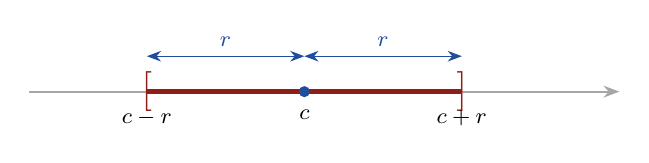
\begin{tikzpicture}[x=1cm,font=\footnotesize]
\draw[nl] (-0.5,0)--(7,0);
\draw[seg] (1,0)--(5,0);
\node[brk] at (1,0){$[$}; \node[brk] at (5,0){$]$};
\fill[cDef] (3,0) circle (2pt);
\node[lab] at (1,0){$c-r$}; \node[lab] at (3,0){$c$}; \node[lab] at (5,0){$c+r$};
\draw[{Stealth[length=1.8mm]}-{Stealth[length=1.8mm]},cDef] (1,0.45)--(3,0.45) node[midway,above]{$r$};
\draw[{Stealth[length=1.8mm]}-{Stealth[length=1.8mm]},cDef] (3,0.45)--(5,0.45) node[midway,above]{$r$};
\end{tikzpicture}
\end{LTR}
\par
وبالمثل: $|x-c|<r\iff x\in\,]c-r;c+r[$ \ ؛ \ \bx{|x-c|\geqslant r\iff x\in\,]-\infty;c-r]\cup[c+r;+\infty[}.
\par
وبالعكس: $x\in[a;b]\iff\left|x-c\right|\leqslant r$ حيث $c=\dfrac{a+b}{2}$ (المركز) و $r=\dfrac{b-a}{2}$ (نصف القطر).
\end{khassia}
\begin{mithal}
\begin{itemize}
\item $|x-3|\leqslant2\iff3-2\leqslant x\leqslant3+2\iff\bx{x\in[1;5]}$.
\item $|x+1|<3\iff-4<x<2\iff\bx{x\in\,]-4;2[}$.
\item $|x-2|>1\iff\bx{x\in\,]-\infty;1[\,\cup\,]3;+\infty[}$.
\item $x\in[-2;5]$: \ $c=\frac{-2+5}{2}=\frac{3}{2}$ و $r=\frac{5-(-2)}{2}=\frac{7}{2}$ ، إذن \bx{x\in[-2;5]\iff\left|x-\tfrac{3}{2}\right|\leqslant\tfrac{7}{2}}.
\end{itemize}
\end{mithal}

\subsection{المعادلات والمتراجحات التي تتضمن قيمة مطلقة}
\begin{khassia}[حالات أساسية ($r>0$)]
\begin{itemize}
\item $|x-c|=r\iff x=c-r$ أو $x=c+r$ \quad ؛ \quad $|A|=0\iff A=0$ \quad ؛ \quad $|A|=k<0$: لا حلول.
\item $|A|=|B|\iff A=B$ أو $A=-B$.
\item $|x-a|=|x-b|$ ($a\neq b$) $\iff d(x;a)=d(x;b)\iff$ \bx{x=\frac{a+b}{2}} (منتصف القطعة).
\item $|x-c|\leqslant r\iff x\in[c-r;c+r]$ \quad ؛ \quad $|x-c|\geqslant r\iff x\in\,]-\infty;c-r]\cup[c+r;+\infty[$.
\end{itemize}
\end{khassia}
\begin{mithal}
\begin{itemize}
\item $|2x-1|=3\iff2x-1=3$ أو $2x-1=-3\iff x=2$ أو $x=-1$ ، إذن \bx{S=\{-1;2\}}.
\item $|x-4|\leqslant\frac{5}{2}\iff4-\frac{5}{2}\leqslant x\leqslant4+\frac{5}{2}$ ، إذن \bx{S=\left[\tfrac{3}{2};\tfrac{13}{2}\right]}.
\item $|x-1|=|x+2|\iff d(x;1)=d(x;-2)\iff x=\frac{1+(-2)}{2}$ ، إذن \bx{S=\left\{-\tfrac{1}{2}\right\}}.
\item $|x+2|\geqslant|x-6|\iff d(x;-2)\geqslant d(x;6)$: $x$ أقرب إلى $6$ أو على نفس البعد؛ المنتصف $\frac{-2+6}{2}=2$ ، إذن \bx{S=[2;+\infty[}.
\end{itemize}
\begin{LTR}\centering
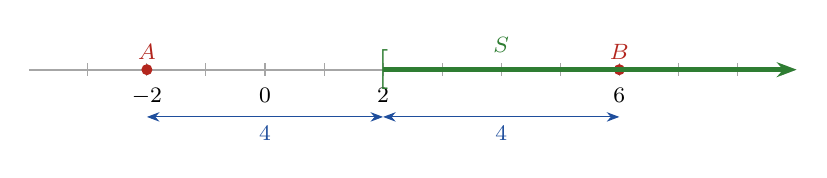
\begin{tikzpicture}[x=0.75cm,font=\footnotesize]
\draw[nl] (-4,0)--(9,0);
\foreach \t in {-3,...,8}\draw[tk] (\t,0.08)--(\t,-0.08);
\foreach \t in {-2,0,2,6}\node[lab] at (\t,0){$\t$};
\fill[cThm] (-2,0) circle (2pt) node[above]{$A$};
\fill[cThm] (6,0) circle (2pt) node[above]{$B$};
\draw[line width=2pt,cRem,-{Stealth[length=2.5mm]}] (2,0)--(9,0);
\node[cRem,font=\Large] at (2,0){$[$};
\node[cRem,above] at (4,0.1){$S$};
\draw[{Stealth[length=1.6mm]}-{Stealth[length=1.6mm]},cDef] (-2,-0.6)--(2,-0.6) node[midway,below]{$4$};
\draw[{Stealth[length=1.6mm]}-{Stealth[length=1.6mm]},cDef] (2,-0.6)--(6,-0.6) node[midway,below]{$4$};
\end{tikzpicture}
\end{LTR}
\end{mithal}

\begin{tariqa}[الحالة العامة: فصل الحالات (جدول)]
\begin{enumerate}
\item نعيّن قيمة $x$ التي تعدم كل عبارة داخل رمز القيمة المطلقة، ونرتبها.
\item ندرس إشارة كل عبارة $ax+b$: إشارة $a$ على يمين $-\frac{b}{a}$ وعكسها على يساره.
\item نكتب العبارة دون رمز القيمة المطلقة على كل مجال (جدول).
\item نحل المعادلة (أو المتراجحة) على كل مجال، ونحتفظ فقط بالحلول التي تنتمي إلى المجال المدروس، ثم نجمعها.
\end{enumerate}
\TAB
\tkzTabInit[lgt=2.2,espcl=3.2]{$x$/0.8,$ax+b$/0.9}{$-\infty$,$-\frac{b}{a}$,$+\infty$}
\tkzTabLine{,\hbox{\ar{عكس إشارة $a$}},z,\hbox{\ar{إشارة $a$}},}
\endTAB
\end{tariqa}
\begin{mithal}[{حل المعادلة $2|x-1|=|x|$}]
$x-1=0\iff x=1$ و $x=0$:
\begin{LTR}\centering
\renewcommand{\arraystretch}{1.35}
\begin{tabular}{|c|c|c|c|}\hline
\rowcolor{cSec!12}$x$ & $]-\infty;0]$ & $[0;1]$ & $[1;+\infty[$\\\hline
$|x|$ & $-x$ & $x$ & $x$\\\hline
$|x-1|$ & $1-x$ & $1-x$ & $x-1$\\\hline
\ar{المعادلة} & $2-2x=-x$ & $2-2x=x$ & $2x-2=x$\\\hline
\ar{الحل} & $x=2\notin\,]-\infty;0]$ & $x=\frac{2}{3}\in[0;1]$ & $x=2\in[1;+\infty[$\\\hline
\end{tabular}
\end{LTR}
\par مجموعة الحلول: \bx{S=\left\{\tfrac{2}{3};2\right\}}.
\end{mithal}

%================================================================
\section{تمارين محلولة متدرجة}
\begin{molahada}[دليل الصعوبة]
$\star$: تطبيق مباشر \qquad $\star\star$: يتطلب ربط خاصيتين \qquad $\star\star\star$: تمرين شامل (نمط الاختبار).
\end{molahada}

\begin{tmr}
[$\star$ \ مجموعات الأعداد] عيّن أصغر مجموعة من بين $\N$ ، $\Z$ ، $\D$ ، $\Q$ ، $\R$ ينتمي إليها كل عدد:
\[ a=\sqrt{49}-10\quad;\quad b=\frac{3}{40}\quad;\quad c=\frac{14}{21}\quad;\quad d=\frac{\left(\sqrt{5}-1\right)\left(\sqrt{5}+1\right)}{8} \]
\[ e=\sqrt{2}\left(1+\frac{1}{1+\sqrt{2}}\right)\quad;\quad f=-\frac{\pi}{4} \]
\end{tmr}
\begin{hal}
\begin{itemize}
\item $a=7-10=-3$ ، إذن \bx{a\in\Z} ($a\notin\N$).
\item $b=\frac{3}{2^{3}\times5}=0{,}075$ ، إذن \bx{b\in\D}.
\item $c=\frac{2}{3}$ (بعد الاختزال على $7$)؛ المقام $3$ ، إذن \bx{c\in\Q} و $c\notin\D$.
\item $d=\frac{5-1}{8}=\frac{1}{2}=0{,}5$ ، إذن \bx{d\in\D}.
\item $\frac{1}{1+\sqrt{2}}=\frac{\sqrt{2}-1}{2-1}=\sqrt{2}-1$ ، ومنه $e=\sqrt{2}\left(1+\sqrt{2}-1\right)=\sqrt{2}\times\sqrt{2}=2$ ، إذن \bx{e\in\N}.
\item $\pi$ عدد أصم، فلو كان $-\frac{\pi}{4}=r\in\Q$ لكان $\pi=-4r\in\Q$: تناقض. إذن \bx{f\in\R} و $f\notin\Q$.
\end{itemize}
\end{hal}

\begin{tmr}
[$\star$ \ $\pgcd$ و $\ppcm$]
\begin{enumerate}
\item حلّل العددين $2520$ و $1848$ إلى جداء عوامل أولية.
\item استنتج $\pgcd(2520;1848)$ و $\ppcm(2520;1848)$ ، ثم اكتب $\frac{1848}{2520}$ على شكل كسر غير قابل للاختزال.
\item تنطلق حافلة من محطة كل $12$ دقيقة وحافلة أخرى كل $18$ دقيقة. انطلقتا معًا على الساعة $7{:}00$. متى تنطلقان معًا مرة أخرى لأول مرة؟
\end{enumerate}
\end{tmr}
\begin{hal}
\QQ{1} $2520=2^{3}\times3^{2}\times5\times7$ \quad ؛ \quad $1848=2^{3}\times3\times7\times11$.
\QQ{2} العوامل المشتركة بأصغر أس: $\pgcd=2^{3}\times3\times7=\bx{168}$. \ كل العوامل بأكبر أس: $\ppcm=2^{3}\times3^{2}\times5\times7\times11=\bx{27720}$.\par
التحقق: $168\times27720=4\,656\,960=2520\times1848$. \quad $\dfrac{1848}{2520}=\dfrac{1848\div168}{2520\div168}=\bx{\frac{11}{15}}$.
\QQ{3} $12=2^{2}\times3$ و $18=2\times3^{2}$ ، إذن $\ppcm(12;18)=2^{2}\times3^{2}=36$. تنطلقان معًا بعد $36$ دقيقة، أي على الساعة \bx{7{:}36}.
\end{hal}

\begin{tmr}
[$\star\star$ \ جذور وقيمة مطلقة] \ ليكن $a=\sqrt{50}-\sqrt{8}\left(\sqrt{2}+1\right)$.
\begin{enumerate}
\item بيّن أن $a=3\sqrt{2}-4$ ، ثم استنتج إشارة $a$.
\item نضع $x=\dfrac{7}{\sqrt{2}+1}$ و $y=\dfrac{1}{\sqrt{2}-1}$. بيّن أن $x-y=2a$ ، ثم قارن $x$ و $y$.
\item اكتب دون رمز القيمة المطلقة: $|a|$ ، $|y-x|$ ، و $A=\left|\sqrt{3}-2\right|+\left|2\sqrt{3}-1\right|-\left|\sqrt{3}-3\right|$.
\end{enumerate}
\end{tmr}
\begin{hal}
\QQ{1} $\sqrt{50}=5\sqrt{2}$ و $\sqrt{8}=2\sqrt{2}$ ، ومنه $a=5\sqrt{2}-2\sqrt{2}\times\sqrt{2}-2\sqrt{2}=5\sqrt{2}-4-2\sqrt{2}=\bx{3\sqrt{2}-4}$.\par
\textbf{الإشارة:} $3\sqrt{2}=\sqrt{18}$ و $4=\sqrt{16}$ ، و $\sqrt{18}>\sqrt{16}$ ، إذن \bx{a>0}.
\QQ{2} بالضرب في المرافق: $x=\dfrac{7\left(\sqrt{2}-1\right)}{2-1}=7\sqrt{2}-7$ و $y=\dfrac{\sqrt{2}+1}{2-1}=\sqrt{2}+1$.\par
$x-y=7\sqrt{2}-7-\sqrt{2}-1=6\sqrt{2}-8=2\left(3\sqrt{2}-4\right)=\bx{2a}$. \ وبما أن $a>0$ فإن $x-y>0$ ، أي \bx{x>y}.
\QQ{3} $a>0$: \ $|a|=\bx{3\sqrt{2}-4}$ \ ؛ \ $y-x=-2a<0$: \ $|y-x|=x-y=\bx{6\sqrt{2}-8}$.\par
$\sqrt{3}<2$: $\left|\sqrt{3}-2\right|=2-\sqrt{3}$ \ ؛ \ $2\sqrt{3}>1$: $\left|2\sqrt{3}-1\right|=2\sqrt{3}-1$ \ ؛ \ $\sqrt{3}<3$: $\left|\sqrt{3}-3\right|=3-\sqrt{3}$.\par
$A=\left(2-\sqrt{3}\right)+\left(2\sqrt{3}-1\right)-\left(3-\sqrt{3}\right)=\bx{2\sqrt{3}-2}$.
\end{hal}

\begin{tmr}
[$\star\star$ \ البرهان على مساواة]
\begin{enumerate}
\item بيّن أن $4+2\sqrt{3}=\left(\sqrt{3}+1\right)^{2}$ و $4-2\sqrt{3}=\left(\sqrt{3}-1\right)^{2}$.
\item استنتج أن $\sqrt{4+2\sqrt{3}}-\sqrt{4-2\sqrt{3}}=2$.
\end{enumerate}
\end{tmr}
\begin{hal}
\QQ{1} $\left(\sqrt{3}+1\right)^{2}=3+2\sqrt{3}+1=\bx{4+2\sqrt{3}}$ \ و \ $\left(\sqrt{3}-1\right)^{2}=3-2\sqrt{3}+1=\bx{4-2\sqrt{3}}$.
\QQ{2} $\sqrt{X^{2}}=|X|$: \ $\sqrt{4+2\sqrt{3}}=\left|\sqrt{3}+1\right|=\sqrt{3}+1$ ، و $\sqrt{4-2\sqrt{3}}=\left|\sqrt{3}-1\right|=\sqrt{3}-1$ (لأن $\sqrt{3}>1$).\par
إذن $\sqrt{4+2\sqrt{3}}-\sqrt{4-2\sqrt{3}}=\left(\sqrt{3}+1\right)-\left(\sqrt{3}-1\right)=\bx{2}$.
\end{hal}

\begin{tmr}
[$\star\star$ \ متباينات شهيرة والمقارنة]
\begin{enumerate}
\item $a$ و $b$ عددان حقيقيان موجبان تمامًا. بيّن أن $\dfrac{a+b}{2}\geqslant\sqrt{ab}$ ، ثم استنتج أنه من أجل كل $a>0$: $a+\dfrac{1}{a}\geqslant2$.
\item $x$ عدد حقيقي موجب تمامًا. نضع $X=\dfrac{x-1}{x}$ و $Y=\dfrac{x}{x+1}$. احسب $X-Y$ ثم قارن $X$ و $Y$.
\item استنتج مقارنة العددين $\sqrt{\dfrac{2023}{2024}}$ و $\sqrt{\dfrac{2024}{2025}}$ (دون آلة حاسبة).
\end{enumerate}
\end{tmr}
\begin{hal}
\QQ{1} ندرس إشارة الفرق: $\dfrac{a+b}{2}-\sqrt{ab}=\dfrac{a-2\sqrt{a}\sqrt{b}+b}{2}=\dfrac{\left(\sqrt{a}-\sqrt{b}\right)^{2}}{2}\geqslant0$ ، إذن \bx{\frac{a+b}{2}\geqslant\sqrt{ab}}.\par
نضع $b=\frac{1}{a}$: \ $\dfrac{a+\frac{1}{a}}{2}\geqslant\sqrt{a\times\frac{1}{a}}=1$ ، ومنه \bx{a+\frac{1}{a}\geqslant2}.
\QQ{2} $X-Y=\dfrac{(x-1)(x+1)-x^{2}}{x(x+1)}=\dfrac{x^{2}-1-x^{2}}{x(x+1)}=\dfrac{-1}{x(x+1)}$. \ بما أن $x>0$ فإن $x(x+1)>0$ ، ومنه $X-Y<0$ ، أي \bx{X<Y}.
\QQ{3} من أجل $x=2024$: $X=\frac{2023}{2024}$ و $Y=\frac{2024}{2025}$ ، إذن $\frac{2023}{2024}<\frac{2024}{2025}$. والعددان موجبان، والجذر التربيعي يحافظ على الترتيب للأعداد الموجبة:
\[ \bx{\sqrt{\frac{2023}{2024}}<\sqrt{\frac{2024}{2025}}} \]
\end{hal}

\begin{tmr}
[$\star\star$ \ الحصر]
\begin{enumerate}
\item $x$ عدد حقيقي حيث: $\dfrac{2}{19}\leqslant\dfrac{2}{2x-3}\leqslant\dfrac{2}{17}$. بيّن أن $10\leqslant x\leqslant11$ ، ثم أعط حصرًا للعدد $11-x$.
\item قارن بين $(11-x)^{1954}$ ، $(11-x)^{1962}$ و $(11-x)^{2024}$.
\item $a$ و $b$ عددان حقيقيان حيث $1<a<2$ و $-3<b<-2$. أعط حصرًا لكل من $3a+b$ ، $1+b^{2}$ و $\dfrac{3a+b}{1+b^{2}}$.
\end{enumerate}
\end{tmr}
\begin{hal}
\QQ{1} الأعداد الثلاثة موجبة تمامًا، وأخذ المقلوب يغيّر اتجاه المتباينة: $\dfrac{17}{2}\leqslant\dfrac{2x-3}{2}\leqslant\dfrac{19}{2}$ ، أي $17\leqslant2x-3\leqslant19$.\par
بإضافة $3$: $20\leqslant2x\leqslant22$ ، وبالقسمة على $2$: \bx{10\leqslant x\leqslant11}.\par
بالضرب في $-1$: $-11\leqslant-x\leqslant-10$ ، وبإضافة $11$: \bx{0\leqslant11-x\leqslant1}.
\QQ{2} نضع $t=11-x$ مع $0\leqslant t\leqslant1$. من أجل عدد بين $0$ و $1$ ، كلما كبر الأس صغرت القوة (نضرب $t\leqslant1$ في $t^{n}\geqslant0$: $t^{n+1}\leqslant t^{n}$):
\[ \bx{(11-x)^{2024}\leqslant(11-x)^{1962}\leqslant(11-x)^{1954}} \]
\QQ{3} $3<3a<6$ و $-3<b<-2$ ، بالجمع: \bx{0<3a+b<4}.\par
$-3<b<-2$ (أعداد سالبة): بالتربيع يتغير الاتجاه: $4<b^{2}<9$ ، ومنه \bx{5<1+b^{2}<10}.\par
$\frac{1}{10}<\frac{1}{1+b^{2}}<\frac{1}{5}$ ، وبما أن $0<3a+b<4$ (أعداد موجبة) فبالضرب: $0\times\frac{1}{10}<\frac{3a+b}{1+b^{2}}<4\times\frac{1}{5}$ ، أي \bx{0<\frac{3a+b}{1+b^{2}}<\frac{4}{5}}.
\end{hal}

\begin{tmr}
[$\star\star$ \ وضعية من الحياة: الحصر] \ قاس تلميذ طول قطعة أرض مستطيلة $L$ وعرضها $\ell$ (بالمتر) فوجد: $12{,}3\leqslant L\leqslant12{,}4$ و $5{,}6\leqslant\ell\leqslant5{,}7$.
\begin{enumerate}
\item أعط حصرًا لمحيط القطعة $P$ ولمساحتها $S$.
\item يريد إحاطتها بسياج سعر المتر منه $850\ DA$. ما هو أقصى مبلغ يلزمه؟
\end{enumerate}
\end{tmr}
\begin{hal}
\QQ{1} $17{,}9\leqslant L+\ell\leqslant18{,}1$ و $P=2(L+\ell)$ ، إذن \bx{35{,}8\leqslant P\leqslant36{,}2} (بالمتر).\par
$S=L\times\ell$ (أعداد موجبة): $12{,}3\times5{,}6\leqslant S\leqslant12{,}4\times5{,}7$ ، أي \bx{68{,}88\leqslant S\leqslant70{,}68} (بالمتر المربع).
\QQ{2} التكلفة $850\times P\leqslant850\times36{,}2=30\,770$. أقصى مبلغ يلزمه هو \bx{30\,770\ DA}.
\end{hal}

\begin{tmr}
[$\star\star$ \ القيم المقربة] \ نعلم أن: $1{,}414<\sqrt{2}<1{,}415$.
\begin{enumerate}
\item أعط حصرًا للعدد $3\sqrt{2}-1$.
\item بيّن أن $\dfrac{1}{\sqrt{2}+1}=\sqrt{2}-1$ ، ثم أعط حصرًا له.
\item استنتج قيمة مقربة بالنقصان وأخرى بالزيادة إلى $10^{-2}$ للعدد $3\sqrt{2}-1$.
\end{enumerate}
\end{tmr}
\begin{hal}
\QQ{1} بالضرب في $3$: $4{,}242<3\sqrt{2}<4{,}245$ ، وبإضافة $-1$: \bx{3{,}242<3\sqrt{2}-1<3{,}245}.
\QQ{2} $\dfrac{1}{\sqrt{2}+1}=\dfrac{\sqrt{2}-1}{\left(\sqrt{2}+1\right)\left(\sqrt{2}-1\right)}=\dfrac{\sqrt{2}-1}{2-1}=\sqrt{2}-1$ ، ومنه \bx{0{,}414<\sqrt{2}-1<0{,}415}.
\QQ{3} $3{,}24<3{,}242<3\sqrt{2}-1<3{,}245<3{,}25$: \ \bx{3{,}24} قيمة مقربة بالنقصان و \bx{3{,}25} قيمة مقربة بالزيادة إلى $10^{-2}$.
\end{hal}

\begin{tmr}
[$\star$ \ المجالات] \ نعتبر المجالين $I=[-6;2]$ و $J=\,]-1;7[$.
\begin{enumerate}
\item مثّل المجالين على مستقيم عددي.
\item عيّن: $I\cap J$ ، $I\cup J$ ، $I\cap\R_{+}$ و $J\cup\R_{-}$.
\end{enumerate}
\end{tmr}
\begin{hal}
\QQ{1}
\begin{LTR}\centering
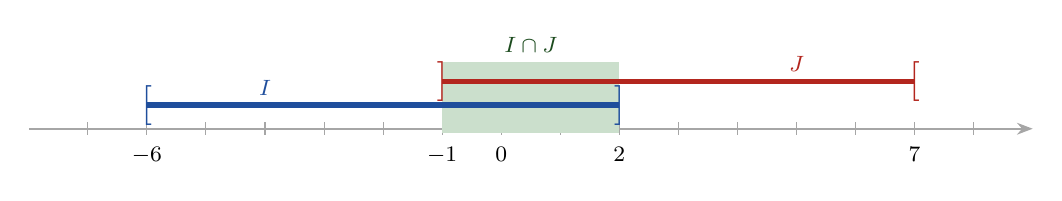
\begin{tikzpicture}[x=0.75cm,font=\footnotesize]
\draw[nl] (-8,0)--(9,0);
\foreach \t in {-7,...,8}\draw[tk] (\t,0.08)--(\t,-0.08);
\foreach \t in {-6,-1,0,2,7}\node[lab] at (\t,0){$\t$};
\fill[cRem!25] (-1,-0.05) rectangle (2,0.85);
\draw[line width=2pt,cDef] (-6,0.3)--(2,0.3);
\node[cDef,font=\Large] at (-6,0.3){$[$}; \node[cDef,font=\Large] at (2,0.3){$]$};
\node[cDef,above] at (-4,0.3){$I$};
\draw[line width=2pt,cThm] (-1,0.6)--(7,0.6);
\node[cThm,font=\Large] at (-1,0.6){$]$}; \node[cThm,font=\Large] at (7,0.6){$[$};
\node[cThm,above] at (5,0.6){$J$};
\node[cRem!60!black,above] at (0.5,0.85){$I\cap J$};
\end{tikzpicture}
\end{LTR}
\QQ{2} \bx{I\cap J=\,]-1;2]} \ ؛ \ \bx{I\cup J=[-6;7[} \ ؛ \ \bx{I\cap\R_{+}=[0;2]} \ ؛ \ \bx{J\cup\R_{-}=\,]-\infty;7[}.
\end{hal}

\begin{tmr}
[$\star\star$ \ المجال، الحصر، المسافة والقيمة المطلقة] \ اكتب كل نص من النصوص الآتية بالصيغ الثلاث الأخرى (مجال، حصر، مسافة، قيمة مطلقة):
\[ x\in\,]1;3[\quad;\quad |x+5|<3\quad;\quad x\in[-3;1]\quad;\quad d(x;-3)\leqslant1\quad;\quad 1\leqslant x\leqslant5\quad;\quad \left|x-\tfrac{1}{2}\right|<4 \]
\end{tmr}
\begin{hal}
\textbf{الطريقة:} من المجال $[a;b]$ نحسب المركز $c=\frac{a+b}{2}$ ونصف القطر $r=\frac{b-a}{2}$ ، ثم نكتب $|x-c|\leqslant r$ (أو $<$ إذا كان المجال مفتوحًا)؛ ومن $|x-c|\leqslant r$ نكتب $c-r\leqslant x\leqslant c+r$.
\begin{center}
\renewcommand{\arraystretch}{1.5}
\begin{tabular}{|>{\centering\arraybackslash}p{0.2\textwidth}|>{\centering\arraybackslash}p{0.22\textwidth}|>{\centering\arraybackslash}p{0.18\textwidth}|>{\centering\arraybackslash}p{0.2\textwidth}|}\hline
\rowcolor{cSec!12}\textbf{المجال} & \textbf{الحصر} & \textbf{المسافة} & \textbf{القيمة المطلقة}\\\hline
$]1;3[$ & $1<x<3$ & $d(x;2)<1$ & $|x-2|<1$\\\hline
$]-8;-2[$ & $-8<x<-2$ & $d(x;-5)<3$ & $|x+5|<3$\\\hline
$[-3;1]$ & $-3\leqslant x\leqslant1$ & $d(x;-1)\leqslant2$ & $|x+1|\leqslant2$\\\hline
$[-4;-2]$ & $-4\leqslant x\leqslant-2$ & $d(x;-3)\leqslant1$ & $|x+3|\leqslant1$\\\hline
$[1;5]$ & $1\leqslant x\leqslant5$ & $d(x;3)\leqslant2$ & $|x-3|\leqslant2$\\\hline
$\left]-\frac{7}{2};\frac{9}{2}\right[$ & $-\frac{7}{2}<x<\frac{9}{2}$ & $d\left(x;\frac{1}{2}\right)<4$ & $\left|x-\frac{1}{2}\right|<4$\\\hline
\end{tabular}
\end{center}
\end{hal}

\begin{tmr}
[$\star\star\star$ \ معادلة بقيمتين مطلقتين] \ حل جبريًا في $\R$ المعادلة: $|2x+5|+|x-9|=12$.
\end{tmr}
\begin{hal}
$2x+5=0\iff x=-\frac{5}{2}$ \ و \ $x-9=0\iff x=9$. نكتب العبارة دون رمز القيمة المطلقة على كل مجال:
\begin{LTR}\centering
\renewcommand{\arraystretch}{1.4}
\begin{tabular}{|c|c|c|c|}\hline
\rowcolor{cSec!12}$x$ & $\left]-\infty;-\frac{5}{2}\right]$ & $\left[-\frac{5}{2};9\right]$ & $[9;+\infty[$\\\hline
$|2x+5|$ & $-2x-5$ & $2x+5$ & $2x+5$\\\hline
$|x-9|$ & $-x+9$ & $-x+9$ & $x-9$\\\hline
$|2x+5|+|x-9|$ & $-3x+4$ & $x+14$ & $3x-4$\\\hline
\end{tabular}
\end{LTR}
\begin{itemize}
\item على $\left]-\infty;-\frac{5}{2}\right]$: $-3x+4=12\iff x=-\frac{8}{3}\approx-2{,}67$ و $-\frac{8}{3}\leqslant-\frac{5}{2}$: \textbf{مقبول}.
\item على $\left[-\frac{5}{2};9\right]$: $x+14=12\iff x=-2$ و $-2\in\left[-\frac{5}{2};9\right]$: \textbf{مقبول}.
\item على $[9;+\infty[$: $3x-4=12\iff x=\frac{16}{3}\approx5{,}33<9$: \textbf{مرفوض}.
\end{itemize}
مجموعة الحلول: \bx{S=\left\{-\tfrac{8}{3};-2\right\}}. \quad (تحقق: $\left|-\frac{1}{3}\right|+\left|-\frac{35}{3}\right|=\frac{36}{3}=12$ \ و \ $|1|+|-11|=12$.)
\end{hal}

\begin{tmr}
[$\star\star\star$ \ القيمة المطلقة والمسافة] \ نعتبر العبارة $E(x)=|x-1|+|x+2|$.
\begin{enumerate}
\item اكتب $E(x)$ دون رمز القيمة المطلقة.
\item حل في $\R$ المعادلة $E(x)=5$.
\item حل في $\R$ المتراجحة $E(x)\leqslant3$ ، ثم فسّر النتيجة باستعمال المسافة.
\end{enumerate}
\end{tmr}
\begin{hal}
\QQ{1}
\begin{LTR}\centering
\renewcommand{\arraystretch}{1.35}
\begin{tabular}{|c|c|c|c|}\hline
\rowcolor{cSec!12}$x$ & $]-\infty;-2]$ & $[-2;1]$ & $[1;+\infty[$\\\hline
$|x-1|$ & $-x+1$ & $-x+1$ & $x-1$\\\hline
$|x+2|$ & $-x-2$ & $x+2$ & $x+2$\\\hline
$E(x)$ & $-2x-1$ & $3$ & $2x+1$\\\hline
\end{tabular}
\end{LTR}
\QQ{2} على $]-\infty;-2]$: $-2x-1=5\iff x=-3$ (مقبول). \ على $[-2;1]$: $3=5$ مستحيل. \ على $[1;+\infty[$: $2x+1=5\iff x=2$ (مقبول). \ إذن \bx{S=\{-3;2\}}.
\QQ{3} على $]-\infty;-2]$: $-2x-1\leqslant3\iff x\geqslant-2$ ، أي $x=-2$. \ على $[-2;1]$: $3\leqslant3$ محققة دائمًا. \ على $[1;+\infty[$: $2x+1\leqslant3\iff x\leqslant1$ ، أي $x=1$. إذن \bx{S=[-2;1]}.\par
\textbf{التفسير:} $E(x)=d(x;1)+d(x;-2)=MA+MB$ حيث $A(1)$ ، $B(-2)$ و $M(x)$. لدينا $AB=3$ ، و $MA+MB=3$ إذا وفقط إذا كانت $M$ على القطعة $[AB]$ ، وإلا فإن $MA+MB>3$.
\begin{LTR}\centering
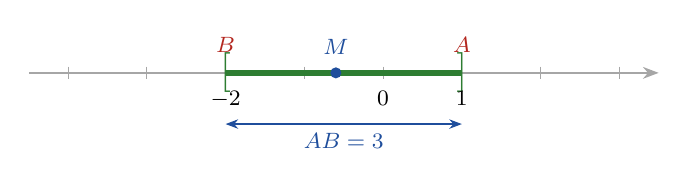
\begin{tikzpicture}[x=1cm,font=\footnotesize]
\draw[nl] (-4.5,0)--(3.5,0);
\foreach \t in {-4,...,3}\draw[tk] (\t,0.08)--(\t,-0.08);
\draw[seg,cRem] (-2,0)--(1,0);
\node[brk,cRem] at (-2,0){$[$}; \node[brk,cRem] at (1,0){$]$};
\node[lab] at (-2,0){$-2$}; \node[lab] at (1,0){$1$}; \node[lab] at (0,0){$0$};
\node[above=4pt,cThm] at (-2,0){$B$}; \node[above=4pt,cThm] at (1,0){$A$};
\fill[cDef] (-0.6,0) circle (2pt) node[above=3pt]{$M$};
\draw[{Stealth[length=1.6mm]}-{Stealth[length=1.6mm]},cDef] (-2,-0.65)--(1,-0.65) node[midway,below]{$AB=3$};
\end{tikzpicture}
\end{LTR}
\end{hal}

\begin{tmr}
[$\star\star\star$ \ تمرين شامل] \ لتكن العبارة $P(x)=\dfrac{1}{2}\sqrt{(2x-6)^{2}}+1$ حيث $x$ عدد حقيقي.
\begin{enumerate}
\item بيّن أن $P(x)=|x-3|+1$.
\item حل في $\R$ المعادلة $P(x)=2$.
\item اكتب عبارة $P(x)$ دون رمز القيمة المطلقة.
\item \begin{sq}
\qa تحقق أن $P\left(\sqrt{7}\right)=4-\sqrt{7}$ و $P\left(\sqrt{11}\right)=\sqrt{11}-2$.
\qb علمًا أن $2{,}64<\sqrt{7}<2{,}65$ و $3{,}31<\sqrt{11}<3{,}32$ ، أعط حصرًا لكل من $P\left(\sqrt{7}\right)$ و $P\left(\sqrt{11}\right)$.
\qc استنتج إشارة الفرق $P\left(\sqrt{11}\right)-P\left(\sqrt{7}\right)$.
\end{sq}
\item بيّن أن: $P(x)\leqslant5$ يكافئ $-1\leqslant x\leqslant7$.
\end{enumerate}
\end{tmr}
\begin{hal}
\QQ{1} $\sqrt{(2x-6)^{2}}=|2x-6|=|2(x-3)|=2|x-3|$ ، ومنه $P(x)=\frac{1}{2}\times2|x-3|+1=\bx{|x-3|+1}$.
\QQ{2} $P(x)=2\iff|x-3|=1\iff x-3=1$ أو $x-3=-1$ ، إذن \bx{S=\{2;4\}}.
\QQ{3} \[ P(x)=\begin{cases} x-2 & \text{\ar{إذا كان}}\ x\geqslant3\\ -x+4 & \text{\ar{إذا كان}}\ x\leqslant3\end{cases} \]
\QQ{4}
\pa $\sqrt{7}<3$ (لأن $7<9$): $P\left(\sqrt{7}\right)=-\sqrt{7}+4=\bx{4-\sqrt{7}}$. \ $\sqrt{11}>3$ (لأن $11>9$): $P\left(\sqrt{11}\right)=\bx{\sqrt{11}-2}$.
\pb $-2{,}65<-\sqrt{7}<-2{,}64$ ، ومنه \bx{1{,}35<P\left(\sqrt{7}\right)<1{,}36}. \ و $3{,}31-2<\sqrt{11}-2<3{,}32-2$ ، أي \bx{1{,}31<P\left(\sqrt{11}\right)<1{,}32}.
\pc $P\left(\sqrt{11}\right)<1{,}32<1{,}35<P\left(\sqrt{7}\right)$ ، إذن \bx{P\left(\sqrt{11}\right)-P\left(\sqrt{7}\right)<0}.
\QQ{5} $P(x)\leqslant5\iff|x-3|\leqslant4\iff3-4\leqslant x\leqslant3+4\iff\bx{-1\leqslant x\leqslant7}$.
\end{hal}

%================================================================
\section{أخطاء شائعة يجب تجنبها}
\begin{BOX}{cThm}{انتبه!}
\begin{enumerate}
\item $\sqrt{a+b}\neq\sqrt{a}+\sqrt{b}$ \ و \ $(a+b)^{2}\neq a^{2}+b^{2}$: \ $\sqrt{9+16}=5\neq7$ \ ؛ \ $(1+2)^{2}=9\neq5$.
\item $\sqrt{x^{2}}=|x|$ وليس $x$: \ $\sqrt{(-3)^{2}}=3$. \ و $(-2)^{4}=16$ بينما $-2^{4}=-16$.
\item الضرب (أو القسمة) في عدد \textbf{سالب} يغيّر اتجاه المتباينة: $-2x<6\iff x>-3$.
\item لا نطرح حصرين طرفًا لطرف: من $2\leqslant x\leqslant3$ و $1\leqslant y\leqslant2$ \textbf{خطأ} $1\leqslant x-y\leqslant1$؛ \textbf{الصحيح}: نحصر $-y$ ثم نجمع: $0\leqslant x-y\leqslant2$.
\item لا نقسم حصرين طرفًا لطرف؛ نحصر المقلوب ثم نضرب (والحدود موجبة).
\item المقلوب لا يطبق إلا على عددين من نفس الإشارة: من $-1<x<2$ ($x\neq0$) لا نستنتج $-1>\frac{1}{x}>\frac{1}{2}$ (مثلًا $x=0{,}1$ يعطي $\frac{1}{x}=10$).
\item التربيع لا يطبق مباشرة إذا تغيّرت الإشارة: من $-3<x<2$ نجد $0\leqslant x^{2}<9$ وليس $9>x^{2}>4$.
\item $|a+b|\neq|a|+|b|$ عمومًا: $|3+(-5)|=2$ بينما $|3|+|-5|=8$. \ و $|x|=x$ فقط إذا كان $x\geqslant0$.
\item لمعرفة إن كان كسر عشريًا نختزله \textbf{أولًا}: $\frac{3}{12}=\frac{1}{4}=0{,}25\in\D$ رغم أن $12=2^{2}\times3$.
\item العدد $1$ ليس أوليًا، والعدد $2$ هو العدد الأولي الزوجي الوحيد.
\item $15\times10^{5}$ ليست كتابة علمية (لأن $15\geqslant10$): الصحيح $1{,}5\times10^{6}$.
\item الرمز $\infty$ دائمًا من جهة مفتوحة: نكتب $[2;+\infty[$ وليس $[2;+\infty]$.
\item حلول $|x-c|\geqslant r$ اتحاد مجالين (وليس تقاطعهما): $|x-2|\geqslant1\iff x\in\,]-\infty;1]\cup[3;+\infty[$.
\item في فصل الحالات، نرفض كل حل لا ينتمي إلى المجال المدروس.
\end{enumerate}
\end{BOX}

%================================================================
\clearpage
\section{خلاصة الطرائق}
\begin{BOX}{cMeth}{الطريقة حسب المطلوب}
\begin{center}
\renewcommand{\arraystretch}{1.3}
\begin{tabular}{|p{0.62\textwidth}|p{0.3\textwidth}|}\hline
\rowcolor{cSec!12} \textbf{الطريقة} & \textbf{المطلوب}\\\hline
نبسّط أولًا، ثم: عدد صحيح؟ كسر غير قابل للاختزال مقامه من الشكل $2^{n}5^{m}$؟ كتابة دورية؟ وإلا فهو أصم (برهان بالخلف). & أصغر مجموعة ينتمي إليها عدد\\\hline
نضرب في $10^{n}$ ($n$ عدد أرقام الدور) ثم نطرح. & كتابة دورية $\to$ كسر\\\hline
نفرض العكس، نستنتج، ونصل إلى تناقض (مثل $\sqrt{2}=\frac{p}{q}$ غير قابل للاختزال). & إثبات أن عددًا أصم\\\hline
القسمة على الأعداد الأولية $p$ حيث $p\leqslant\sqrt{n}$. & هل $n$ أولي؟\\\hline
التحليل: المشتركة بأصغر أس / الكل بأكبر أس؛ أو خوارزمية إقليدس؛ و $\pgcd\times\ppcm=ab$. & $\pgcd$ ، $\ppcm$ ، اختزال كسر\\\hline
قواعد القوى، $\sqrt{ab}=\sqrt{a}\sqrt{b}$ ، $\sqrt{a^{2}}=|a|$ ، الضرب في المرافق. & تبسيط عبارة بقوى أو جذور\\\hline
$a\times10^{n}$ مع $1\leqslant a<10$؛ رتبة المقدار: ندوّر $a$ إلى الوحدة. & كتابة علمية، رتبة مقدار\\\hline
نحوّل طرفًا إلى الآخر، أو الطرفين إلى عبارة واحدة، أو $A-B=0$ ، أو $A^{2}=B^{2}$ مع $A,B\geqslant0$. & إثبات مساواة\\\hline
إشارة الفرق؛ المربعان (عددان موجبان)؛ المقلوبان (نفس الإشارة)؛ $\frac{a}{b}$ و $1$؛ عدد وسيط. & مقارنة عددين\\\hline
نجمع الحصرين؛ نحصر $-y$ ثم نجمع؛ نحصر $\frac{1}{y}$ ثم نضرب (حدود موجبة). & حصر $x+y$ ، $x-y$ ، $xy$ ، $\frac{x}{y}$\\\hline
من حصر سعته $10^{-n}$: الحد الأدنى بالنقصان، الحد الأعلى بالزيادة؛ التدوير حسب الرقم الموالي ($\geqslant5$ أو $<5$). & قيمة مقربة، تدوير\\\hline
نمثل المجالين على نفس المستقيم ونقرأ الجزء المشترك أو كل الجزء الملوّن. & $I\cap J$ ، $I\cup J$\\\hline
المركز $c=\frac{a+b}{2}$ ونصف القطر $r=\frac{b-a}{2}$: $|x-c|\leqslant r\iff x\in[c-r;c+r]$. & مجال $\leftrightarrow$ قيمة مطلقة\\\hline
نحدد إشارة ما داخل القيمة المطلقة: $|A|=A$ إذا $A\geqslant0$ و $|A|=-A$ إذا $A\leqslant0$. & كتابة دون رمز القيمة المطلقة\\\hline
$|x-c|=r$: $x=c\pm r$؛ $|A|=|B|$: $A=\pm B$؛ $|x-a|=|x-b|$: المنتصف $\frac{a+b}{2}$. & معادلة بقيمة مطلقة\\\hline
جدول فصل الحالات، الحل على كل مجال، رفض الحلول خارج المجال، ثم الاتحاد. & معادلة أو متراجحة بعدة قيم مطلقة\\\hline
\end{tabular}
\end{center}
\end{BOX}
\end{document}
